%%%%%%%%%%%%%%%%%%%%%%%%%%%%%%%%%%%%%%%%%
% Masters/Doctoral Thesis 
% LaTeX Template
% Version 2.4 (22/11/16)
%
% This template has been downloaded from:
% http://www.LaTeXTemplates.com
%
% Version 2.x major modifications by:
% Vel (vel@latextemplates.com)
%
% This template is based on a template by:
% Steve Gunn (http://users.ecs.soton.ac.uk/srg/softwaretools/document/templates/)
% Sunil Patel (http://www.sunilpatel.co.uk/thesis-template/)
%
% Template license:
% CC BY-NC-SA 3.0 (http://creativecommons.org/licenses/by-nc-sa/3.0/)
%
%%%%%%%%%%%%%%%%%%%%%%%%%%%%%%%%%%%%%%%%%

%----------------------------------------------------------------------------------------
%	PACKAGES AND OTHER DOCUMENT CONFIGURATIONS
%----------------------------------------------------------------------------------------

\documentclass[
11pt, % The default document font size, options: 10pt, 11pt, 12pt
%oneside, % Two side (alternating margins) for binding by default, uncomment to switch to one side
english, % ngerman for German
singlespacing, % Single line spacing, alternatives: onehalfspacing or doublespacing
%draft, % Uncomment to enable draft mode (no pictures, no links, overfull hboxes indicated)
%nolistspacing, % If the document is onehalfspacing or doublespacing, uncomment this to set spacing in lists to single
%liststotoc, % Uncomment to add the list of figures/tables/etc to the table of contents
%toctotoc, % Uncomment to add the main table of contents to the table of contents
%parskip, % Uncomment to add space between paragraphs
%nohyperref, % Uncomment to not load the hyperref package
headsepline, % Uncomment to get a line under the header
%chapterinoneline, % Uncomment to place the chapter title next to the number on one line
%consistentlayout, % Uncomment to change the layout of the declaration, abstract and acknowledgements pages to match the default layout
]{MastersDoctoralThesis} % The class file specifying the document structure

\usepackage[hyphens]{url} % Required for line breaking in urls

\usepackage{pdfpages} % Required for including pdfs

\usepackage{float} % Required for fixing tables/figures in place 

\usepackage{threeparttable} % Required for my tables

\usepackage{graphicx} % Required for adding jpg images

\usepackage{textcomp} % Required for µ

\usepackage[utf8]{inputenc} % Required for inputting international characters
\usepackage[T1]{fontenc} % Output font encoding for international characters

\usepackage{mathtools} % Used for mathematical formulas

\usepackage{palatino} % Use the Palatino font by default

\usepackage[backend=biber,style=authoryear,natbib=true]{biblatex} % Use the bibtex backend with the authoryear citation style (which resembles APA)

\addbibresource{bibliography.bib} % The filename of the bibliography

\usepackage[autostyle=true]{csquotes} % Required to generate language-dependent quotes in the bibliography

%----------------------------------------------------------------------------------------
%	MARGIN SETTINGS
%----------------------------------------------------------------------------------------

\geometry{
	paper=a4paper, % Change to letterpaper for US letter
	inner=2.5cm, % Inner margin
	outer=3.8cm, % Outer margin
	bindingoffset=.5cm, % Binding offset
	top=1.5cm, % Top margin
	bottom=1.5cm, % Bottom margin
	%showframe, % Uncomment to show how the type block is set on the page
}

%----------------------------------------------------------------------------------------
%	THESIS INFORMATION
%----------------------------------------------------------------------------------------

\thesistitle{Machine Learning for Indoor Positioning} % Your thesis title, this is used in the title and abstract, print it elsewhere with \ttitle
\supervisor{Dr. Zhongliang \textsc{Zhao}} % Your supervisor's name, this is used in the title page, print it elsewhere with \supname
\newcommand{\supername}{Jose Luis \textsc{Carrera}}
\examiner{Prof. Dr. Torsten \textsc{Braun}} % Your examiner's name, this is not currently used anywhere in the template, print it elsewhere with \examname
\degree{Bachelor of Science} % Your degree name, this is used in the title page and abstract, print it elsewhere with \degreename
\author{Joel \textsc{Niklaus}} % Your name, this is used in the title page and abstract, print it elsewhere with \authorname
\addresses{} % Your address, this is not currently used anywhere in the template, print it elsewhere with \addressname

\subject{Machine Learning} % Your subject area, this is not currently used anywhere in the template, print it elsewhere with \subjectname
\keywords{Computer Science, Machine Learning, Indoor Localization, Indoor Positioning, Wireless, Smartphones,} % Keywords for your thesis, this is not currently used anywhere in the template, print it elsewhere with \keywordnames
\university{\href{http://www.unibe.ch}{University of Bern}} % Your university's name and URL, this is used in the title page and abstract, print it elsewhere with \univname
\department{\href{http://inf.unibe.ch}{Institute of Computer Science}} % Your department's name and URL, this is used in the title page and abstract, print it elsewhere with \deptname
\group{\href{http://cds.unibe.ch}{Communication and Distributed Systems Research Group}} % Your research group's name and URL, this is used in the title page, print it elsewhere with \groupname
\faculty{\href{http://philnat.unibe.ch}{Faculty of Science}} % Your faculty's name and URL, this is used in the title page and abstract, print it elsewhere with \facname

\AtBeginDocument{
    \hypersetup{pdftitle=\ttitle} % Set the PDF's title to your title
    \hypersetup{pdfauthor=\authorname} % Set the PDF's author to your name
    \hypersetup{pdfkeywords=\keywordnames} % Set the PDF's keywords to your keywords
}

\begin{document}

% Define some commands to keep the formatting separated from the content 
\newcommand{\keyword}[1]{\textbf{#1}}
\newcommand{\tabhead}[1]{\textbf{#1}}
\newcommand{\code}[1]{\texttt{#1}}
\newcommand{\file}[1]{\texttt{\bfseries#1}}
\newcommand{\option}[1]{\texttt{\itshape#1}}

\frontmatter % Use roman page numbering style (i, ii, iii, iv...) for the pre-content pages

\pagestyle{plain} % Default to the plain heading style until the thesis style is called for the body content

%----------------------------------------------------------------------------------------
%	TITLE PAGE
%----------------------------------------------------------------------------------------

\begin{titlepage}
\begin{center}

\vspace*{.06\textheight}
{\scshape\LARGE \univname\par}\vspace{0.5cm} % University name
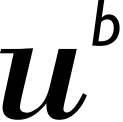
\includegraphics[width=20mm]{Figures/UniversityCrest.png}\\[1.0cm] % University/department logo
\textsc{\Large Bachelor Thesis}\\[0.5cm] % Thesis type

\HRule \\[0.4cm] % Horizontal line
{\huge \bfseries \ttitle\par}\vspace{0.4cm} % Thesis title
\HRule \\[1.5cm] % Horizontal line
 
\begin{minipage}[t]{0.4\textwidth}
\begin{flushleft} \large
\emph{Author:}\\
\href{http://www.joelniklaus.ch}{\authorname} % Author name - remove the \href bracket to remove the link
\end{flushleft}
\end{minipage}
\begin{minipage}[t]{0.4\textwidth}
\begin{flushright} \large
\emph{Supervisors:} \\
\href{http://www.inf.unibe.ch/ueber_uns/personen/prof_dr_braun_torsten/index_ger.html}{\examname} \\ % Examiner name - remove the \href bracket to remove the link  
\href{http://www.inf.unibe.ch/ueber_uns/personen/dr_zhao_zhongliang/index_ger.html}{\supname} \\ % Supervisor name - remove the \href bracket to remove the link  
\href{http://www.inf.unibe.ch/ueber_uns/personen/carrera_jos_luis/index_ger.html}{\supername} % Supervisor name - remove the \href bracket to remove the link
\end{flushright}
\end{minipage}\\[3cm]
 
\vfill

\large \textit{A thesis submitted in fulfillment of the requirements\\ for the degree of \degreename}\\[0.3cm] % University requirement text
\textit{in the}\\[0.4cm]
\groupname\\\deptname\\[2cm] % Research group name and department name
 
\vfill

{\large \today}\\[4cm] % Date
 
\vfill
\end{center}
\end{titlepage}

%----------------------------------------------------------------------------------------
%	DECLARATION PAGE
%----------------------------------------------------------------------------------------

\begin{declaration}
\addchaptertocentry{\authorshipname} % Add the declaration to the table of contents
\noindent I, \authorname, declare that this thesis titled, \enquote{\ttitle} and the work presented in it are my own. I confirm that:

\begin{itemize} 
\item This work was done wholly or mainly while in candidature for a research degree at this University.
\item Where any part of this thesis has previously been submitted for a degree or any other qualification at this University or any other institution, this has been clearly stated.
\item Where I have consulted the published work of others, this is always clearly attributed.
\item Where I have quoted from the work of others, the source is always given. With the exception of such quotations, this thesis is entirely my own work.
\item I have acknowledged all main sources of help.
\item Where the thesis is based on work done by myself jointly with others, I have made clear exactly what was done by others and what I have contributed myself.\\
\end{itemize}
 
\noindent Signed:\\
\rule[0.5em]{25em}{0.5pt} % This prints a line for the signature
 
\noindent Date:\\
\rule[0.5em]{25em}{0.5pt} % This prints a line to write the date
\end{declaration}

\cleardoublepage

%----------------------------------------------------------------------------------------
%	QUOTATION PAGE
%----------------------------------------------------------------------------------------

\vspace*{0.2\textheight}

\noindent\enquote{\itshape In a world that's changing really quickly, the only strategy that is guaranteed to fail is not taking risks.}\bigbreak

\hfill Mark Zuckerberg

%----------------------------------------------------------------------------------------
%	ABSTRACT PAGE
%----------------------------------------------------------------------------------------

\begin{abstract}
\addchaptertocentry{\abstractname} % Add the abstract to the table of contents
Nowadays, smartphones can collect huge amounts of data in their surrounding environment with the help of highly accurate sensors. Since the combination of the Received Signal Strengths of surrounding Access Points and sensor data is assumed to be unique in every location, it should be possible to use this information to accurately predict a smartphone's location. As it is very difficult to derive the correlation between these values, we must use machine learning methods. As part of this project, we have developed an Android application that is able to distinguish between rooms on a floor and special landmarks within a room. This has been accomplished using machine learning methods based on the Java library Weka. Ultimately, we  hope to include this application into an indoor tracking system in order to improve its accuracy.
\end{abstract}

%----------------------------------------------------------------------------------------
%	ACKNOWLEDGEMENTS
%----------------------------------------------------------------------------------------

\begin{acknowledgements}
\addchaptertocentry{\acknowledgementname} % Add the acknowledgements to the table of contents
On this page I want to thank every person who helped me in any way in completing this thesis. In particular I want to give sincere thanks to my supervisors \examname, \supname \ and \supername \ for their help and support during my project. Furthermore, I yield Melissa CHANG and Catriona REID special thanks for proof reading my thesis and helping me greatly with the English language. In addition I want to thank my flatmates in Exeter and Bern warmly for their patience while I was disturbing them by conducting my experiments in the living room. Last but not least many thanks to my parents, siblings and friends for their emotional support.
\end{acknowledgements}

%----------------------------------------------------------------------------------------
%	LIST OF CONTENTS/FIGURES/TABLES PAGES
%----------------------------------------------------------------------------------------

\tableofcontents % Prints the main table of contents

\listoffigures % Prints the list of figures

\listoftables % Prints the list of tables

%----------------------------------------------------------------------------------------
%	ABBREVIATIONS
%----------------------------------------------------------------------------------------

\begin{abbreviations}{ll} % Include a list of abbreviations (a table of two columns)

\textbf{ML} & \textbf{M}achine \textbf{L}earning\\
\textbf{IL} & \textbf{I}ndoor \textbf{L}ocalization\\
\textbf{IP} & \textbf{I}ndoor \textbf{P}ositioning\\
\textbf{ITS} & \textbf{I}ndoor \textbf{T}racking \textbf{S}ystem\\
\textbf{RSS} & \textbf{R}eceived \textbf{S}ignal \textbf{S}trength\\
\textbf{Indoloc} & This \textbf{Indo}or \textbf{Loc}alization System\\
\textbf{KNN} & \textbf{K} \textbf{N}earest \textbf{N}eighbour\\

\end{abbreviations}


% %----------------------------------------------------------------------------------------
% %	DEFINITIONS
% %----------------------------------------------------------------------------------------

% \begin{definitions}{ll} % Include a list of definitions (a table of two columns)

% \textbf{Features} & In a Machine Learning project a feature denotes an attribute of the data which helps to make the prediction.\\


% \end{definitions}


%----------------------------------------------------------------------------------------
%	PHYSICAL CONSTANTS/OTHER DEFINITIONS
%----------------------------------------------------------------------------------------

%\begin{constants}{lr@{${}={}$}l} % The list of physical constants is a three column table

% The \SI{}{} command is provided by the siunitx package, see its documentation for instructions on how to use it

%Speed of Light & $c_{0}$ & \SI{2.99792458e8}{\meter\per\second} (exact)\\
%Constant Name & $Symbol$ & $Constant Value$ with units\\

%\end{constants}

%----------------------------------------------------------------------------------------
%	SYMBOLS
%----------------------------------------------------------------------------------------

%\begin{symbols}{lll} % Include a list of Symbols (a three column table)
%
%$a$ & distance & \si{\meter} \\
%$P$ & power & \si{\watt} (\si{\joule\per\second}) \\
%%Symbol & Name & Unit \\
%
%\addlinespace % Gap to separate the Roman symbols from the Greek
%
%$\omega$ & angular frequency & \si{\radian} \\
%
%\end{symbols}

%----------------------------------------------------------------------------------------
%	DEDICATION
%----------------------------------------------------------------------------------------

%\dedicatory{This thesis is dedicated to you the reader.} 
\dedicatory{This thesis is dedicated to everyone who helped me on the project, except for that guy who yelled at me in Migros when I was  seven because he thought I was being "too rowdy".\\[0.5cm]You're an asshole, sir.}

%----------------------------------------------------------------------------------------
%	THESIS CONTENT - CHAPTERS
%----------------------------------------------------------------------------------------

\mainmatter % Begin numeric (1,2,3...) page numbering

\pagestyle{thesis} % Return the page headers back to the "thesis" style

% Include the chapters of the thesis as separate files from the Chapters folder
% Uncomment the lines as you write the chapters

%% Chapter 0

\chapter{Chapter Title Here} % Main chapter title

\label{Chapter0} % For referencing the chapter elsewhere, use \ref{Chapter0} 

%----------------------------------------------------------------------------------------

% Define some commands to keep the formatting separated from the content 
\newcommand{\keyword}[1]{\textbf{#1}}
\newcommand{\tabhead}[1]{\textbf{#1}}
\newcommand{\code}[1]{\texttt{#1}}
\newcommand{\file}[1]{\texttt{\bfseries#1}}
\newcommand{\option}[1]{\texttt{\itshape#1}}

%----------------------------------------------------------------------------------------

\section{Welcome and Thank You}
Welcome to this \LaTeX{} Thesis Template, a beautiful and easy to use template for writing a thesis using the \LaTeX{} typesetting system.
\cite{Reference1}

If you are writing a thesis (or will be in the future) and its subject is technical or mathematical (though it doesn't have to be), then creating it in \LaTeX{} is highly recommended as a way to make sure you can just get down to the essential writing without having to worry over formatting or wasting time arguing with your word processor.

\LaTeX{} is easily able to professionally typeset documents that run to hundreds or thousands of pages long. With simple mark-up commands, it automatically sets out the table of contents, margins, page headers and footers and keeps the formatting consistent and beautiful. One of its main strengths is the way it can easily typeset mathematics, even \emph{heavy} mathematics. Even if those equations are the most horribly twisted and most difficult mathematical problems that can only be solved on a super-computer, you can at least count on \LaTeX{} to make them look stunning.

%----------------------------------------------------------------------------------------

\section{Learning \LaTeX{}}

\LaTeX{} is not a \textsc{wysiwyg} (What You See is What You Get) program, unlike word processors such as Microsoft Word or Apple's Pages. Instead, a document written for \LaTeX{} is actually a simple, plain text file that contains \emph{no formatting}. You tell \LaTeX{} how you want the formatting in the finished document by writing in simple commands amongst the text, for example, if I want to use \emph{italic text for emphasis}, I write the \verb|\emph{text}| command and put the text I want in italics in between the curly braces. This means that \LaTeX{} is a \enquote{mark-up} language, very much like HTML.

\subsection{A (not so short) Introduction to \LaTeX{}}

If you are new to \LaTeX{}, there is a very good eBook -- freely available online as a PDF file -- called, \enquote{The Not So Short Introduction to \LaTeX{}}. The book's title is typically shortened to just \emph{lshort}. You can download the latest version (as it is occasionally updated) from here:
\url{http://www.ctan.org/tex-archive/info/lshort/english/lshort.pdf}

It is also available in several other languages. Find yours from the list on this page: \url{http://www.ctan.org/tex-archive/info/lshort/}

It is recommended to take a little time out to learn how to use \LaTeX{} by creating several, small `test' documents, or having a close look at several templates on:\\ 
\url{http://www.LaTeXTemplates.com}\\ 
Making the effort now means you're not stuck learning the system when what you \emph{really} need to be doing is writing your thesis.

\subsection{A Short Math Guide for \LaTeX{}}

If you are writing a technical or mathematical thesis, then you may want to read the document by the AMS (American Mathematical Society) called, \enquote{A Short Math Guide for \LaTeX{}}. It can be found online here:
\url{http://www.ams.org/tex/amslatex.html}
under the \enquote{Additional Documentation} section towards the bottom of the page.

\subsection{Common \LaTeX{} Math Symbols}
There are a multitude of mathematical symbols available for \LaTeX{} and it would take a great effort to learn the commands for them all. The most common ones you are likely to use are shown on this page:
\url{http://www.sunilpatel.co.uk/latex-type/latex-math-symbols/}

You can use this page as a reference or crib sheet, the symbols are rendered as large, high quality images so you can quickly find the \LaTeX{} command for the symbol you need.

\subsection{\LaTeX{} on a Mac}
 
The \LaTeX{} distribution is available for many systems including Windows, Linux and Mac OS X. The package for OS X is called MacTeX and it contains all the applications you need -- bundled together and pre-customized -- for a fully working \LaTeX{} environment and work flow.
 
MacTeX includes a custom dedicated \LaTeX{} editor called TeXShop for writing your `\file{.tex}' files and BibDesk: a program to manage your references and create your bibliography section just as easily as managing songs and creating playlists in iTunes.

%----------------------------------------------------------------------------------------

\section{Getting Started with this Template}

If you are familiar with \LaTeX{}, then you should explore the directory structure of the template and then proceed to place your own information into the \emph{THESIS INFORMATION} block of the \file{main.tex} file. You can then modify the rest of this file to your unique specifications based on your degree/university. Section \ref{FillingFile} on page \pageref{FillingFile} will help you do this. Make sure you also read section \ref{ThesisConventions} about thesis conventions to get the most out of this template.

If you are new to \LaTeX{} it is recommended that you carry on reading through the rest of the information in this document.

Before you begin using this template you should ensure that its style complies with the thesis style guidelines imposed by your institution. In most cases this template style and layout will be suitable. If it is not, it may only require a small change to bring the template in line with your institution's recommendations. These modifications will need to be done on the \file{MastersDoctoralThesis.cls} file.

\subsection{About this Template}

This \LaTeX{} Thesis Template is originally based and created around a \LaTeX{} style file created by Steve R.\ Gunn from the University of Southampton (UK), department of Electronics and Computer Science. You can find his original thesis style file at his site, here:
\url{http://www.ecs.soton.ac.uk/~srg/softwaretools/document/templates/}

Steve's \file{ecsthesis.cls} was then taken by Sunil Patel who modified it by creating a skeleton framework and folder structure to place the thesis files in. The resulting template can be found on Sunil's site here:
\url{http://www.sunilpatel.co.uk/thesis-template}

Sunil's template was made available through \url{http://www.LaTeXTemplates.com} where it was modified many times based on user requests and questions. Version 2.0 and onwards of this template represents a major modification to Sunil's template and is, in fact, hardly recognisable. The work to make version 2.0 possible was carried out by \href{mailto:vel@latextemplates.com}{Vel} and Johannes Böttcher.

%----------------------------------------------------------------------------------------

\section{What this Template Includes}

\subsection{Folders}

This template comes as a single zip file that expands out to several files and folders. The folder names are mostly self-explanatory:

\keyword{Appendices} -- this is the folder where you put the appendices. Each appendix should go into its own separate \file{.tex} file. An example and template are included in the directory.

\keyword{Chapters} -- this is the folder where you put the thesis chapters. A thesis usually has about six chapters, though there is no hard rule on this. Each chapter should go in its own separate \file{.tex} file and they can be split as:
\begin{itemize}
\item Chapter 1: Introduction to the thesis topic
\item Chapter 2: Background information and theory
\item Chapter 3: (Laboratory) experimental setup
\item Chapter 4: Details of experiment 1
\item Chapter 5: Details of experiment 2
\item Chapter 6: Discussion of the experimental results
\item Chapter 7: Conclusion and future directions
\end{itemize}
This chapter layout is specialised for the experimental sciences, your discipline may be different.

\keyword{Figures} -- this folder contains all figures for the thesis. These are the final images that will go into the thesis document.

\subsection{Files}

Included are also several files, most of them are plain text and you can see their contents in a text editor. After initial compilation, you will see that more auxiliary files are created by \LaTeX{} or BibTeX and which you don't need to delete or worry about:

\keyword{example.bib} -- this is an important file that contains all the bibliographic information and references that you will be citing in the thesis for use with BibTeX. You can write it manually, but there are reference manager programs available that will create and manage it for you. Bibliographies in \LaTeX{} are a large subject and you may need to read about BibTeX before starting with this. Many modern reference managers will allow you to export your references in BibTeX format which greatly eases the amount of work you have to do.

\keyword{MastersDoctoralThesis.cls} -- this is an important file. It is the class file that tells \LaTeX{} how to format the thesis. 

\keyword{main.pdf} -- this is your beautifully typeset thesis (in the PDF file format) created by \LaTeX{}. It is supplied in the PDF with the template and after you compile the template you should get an identical version.

\keyword{main.tex} -- this is an important file. This is the file that you tell \LaTeX{} to compile to produce your thesis as a PDF file. It contains the framework and constructs that tell \LaTeX{} how to layout the thesis. It is heavily commented so you can read exactly what each line of code does and why it is there. After you put your own information into the \emph{THESIS INFORMATION} block -- you have now started your thesis!

Files that are \emph{not} included, but are created by \LaTeX{} as auxiliary files include:

\keyword{main.aux} -- this is an auxiliary file generated by \LaTeX{}, if it is deleted \LaTeX{} simply regenerates it when you run the main \file{.tex} file.

\keyword{main.bbl} -- this is an auxiliary file generated by BibTeX, if it is deleted, BibTeX simply regenerates it when you run the \file{main.aux} file. Whereas the \file{.bib} file contains all the references you have, this \file{.bbl} file contains the references you have actually cited in the thesis and is used to build the bibliography section of the thesis.

\keyword{main.blg} -- this is an auxiliary file generated by BibTeX, if it is deleted BibTeX simply regenerates it when you run the main \file{.aux} file.

\keyword{main.lof} -- this is an auxiliary file generated by \LaTeX{}, if it is deleted \LaTeX{} simply regenerates it when you run the main \file{.tex} file. It tells \LaTeX{} how to build the \emph{List of Figures} section.

\keyword{main.log} -- this is an auxiliary file generated by \LaTeX{}, if it is deleted \LaTeX{} simply regenerates it when you run the main \file{.tex} file. It contains messages from \LaTeX{}, if you receive errors and warnings from \LaTeX{}, they will be in this \file{.log} file.

\keyword{main.lot} -- this is an auxiliary file generated by \LaTeX{}, if it is deleted \LaTeX{} simply regenerates it when you run the main \file{.tex} file. It tells \LaTeX{} how to build the \emph{List of Tables} section.

\keyword{main.out} -- this is an auxiliary file generated by \LaTeX{}, if it is deleted \LaTeX{} simply regenerates it when you run the main \file{.tex} file.

So from this long list, only the files with the \file{.bib}, \file{.cls} and \file{.tex} extensions are the most important ones. The other auxiliary files can be ignored or deleted as \LaTeX{} and BibTeX will regenerate them.

%----------------------------------------------------------------------------------------

\section{Filling in Your Information in the \file{main.tex} File}\label{FillingFile}

You will need to personalise the thesis template and make it your own by filling in your own information. This is done by editing the \file{main.tex} file in a text editor or your favourite LaTeX environment.

Open the file and scroll down to the third large block titled \emph{THESIS INFORMATION} where you can see the entries for \emph{University Name}, \emph{Department Name}, etc \ldots

Fill out the information about yourself, your group and institution. You can also insert web links, if you do, make sure you use the full URL, including the \code{http://} for this. If you don't want these to be linked, simply remove the \verb|\href{url}{name}| and only leave the name.

When you have done this, save the file and recompile \code{main.tex}. All the information you filled in should now be in the PDF, complete with web links. You can now begin your thesis proper!

%----------------------------------------------------------------------------------------

\section{The \code{main.tex} File Explained}

The \file{main.tex} file contains the structure of the thesis. There are plenty of written comments that explain what pages, sections and formatting the \LaTeX{} code is creating. Each major document element is divided into commented blocks with titles in all capitals to make it obvious what the following bit of code is doing. Initially there seems to be a lot of \LaTeX{} code, but this is all formatting, and it has all been taken care of so you don't have to do it.

Begin by checking that your information on the title page is correct. For the thesis declaration, your institution may insist on something different than the text given. If this is the case, just replace what you see with what is required in the \emph{DECLARATION PAGE} block.

Then comes a page which contains a funny quote. You can put your own, or quote your favourite scientist, author, person, and so on. Make sure to put the name of the person who you took the quote from.

Following this is the abstract page which summarises your work in a condensed way and can almost be used as a standalone document to describe what you have done. The text you write will cause the heading to move up so don't worry about running out of space.

Next come the acknowledgements. On this page, write about all the people who you wish to thank (not forgetting parents, partners and your advisor/supervisor).

The contents pages, list of figures and tables are all taken care of for you and do not need to be manually created or edited. The next set of pages are more likely to be optional and can be deleted since they are for a more technical thesis: insert a list of abbreviations you have used in the thesis, then a list of the physical constants and numbers you refer to and finally, a list of mathematical symbols used in any formulae. Making the effort to fill these tables means the reader has a one-stop place to refer to instead of searching the internet and references to try and find out what you meant by certain abbreviations or symbols.

The list of symbols is split into the Roman and Greek alphabets. Whereas the abbreviations and symbols ought to be listed in alphabetical order (and this is \emph{not} done automatically for you) the list of physical constants should be grouped into similar themes.

The next page contains a one line dedication. Who will you dedicate your thesis to?

Finally, there is the block where the chapters are included. Uncomment the lines (delete the \code{\%} character) as you write the chapters. Each chapter should be written in its own file and put into the \emph{Chapters} folder and named \file{Chapter1}, \file{Chapter2}, etc\ldots Similarly for the appendices, uncomment the lines as you need them. Each appendix should go into its own file and placed in the \emph{Appendices} folder.

After the preamble, chapters and appendices finally comes the bibliography. The bibliography style (called \option{authoryear}) is used for the bibliography and is a fully featured style that will even include links to where the referenced paper can be found online. Do not underestimate how grateful your reader will be to find that a reference to a paper is just a click away. Of course, this relies on you putting the URL information into the BibTeX file in the first place.

%----------------------------------------------------------------------------------------

\section{Thesis Features and Conventions}\label{ThesisConventions}

To get the best out of this template, there are a few conventions that you may want to follow.

One of the most important (and most difficult) things to keep track of in such a long document as a thesis is consistency. Using certain conventions and ways of doing things (such as using a Todo list) makes the job easier. Of course, all of these are optional and you can adopt your own method.

\subsection{Printing Format}

This thesis template is designed for double sided printing (i.e. content on the front and back of pages) as most theses are printed and bound this way. Switching to one sided printing is as simple as uncommenting the \option{oneside} option of the \code{documentclass} command at the top of the \file{main.tex} file. You may then wish to adjust the margins to suit specifications from your institution.

The headers for the pages contain the page number on the outer side (so it is easy to flick through to the page you want) and the chapter name on the inner side.

The text is set to 11 point by default with single line spacing, again, you can tune the text size and spacing should you want or need to using the options at the very start of \file{main.tex}. The spacing can be changed similarly by replacing the \option{singlespacing} with \option{onehalfspacing} or \option{doublespacing}.

\subsection{Using US Letter Paper}

The paper size used in the template is A4, which is the standard size in Europe. If you are using this thesis template elsewhere and particularly in the United States, then you may have to change the A4 paper size to the US Letter size. This can be done in the margins settings section in \file{main.tex}.

Due to the differences in the paper size, the resulting margins may be different to what you like or require (as it is common for institutions to dictate certain margin sizes). If this is the case, then the margin sizes can be tweaked by modifying the values in the same block as where you set the paper size. Now your document should be set up for US Letter paper size with suitable margins.

\subsection{References}

The \code{biblatex} package is used to format the bibliography and inserts references such as this one \parencite{Reference1}. The options used in the \file{main.tex} file mean that the in-text citations of references are formatted with the author(s) listed with the date of the publication. Multiple references are separated by semicolons (e.g. \parencite{Reference2, Reference1}) and references with more than three authors only show the first author with \emph{et al.} indicating there are more authors (e.g. \parencite{Reference3}). This is done automatically for you. To see how you use references, have a look at the \file{Chapter1.tex} source file. Many reference managers allow you to simply drag the reference into the document as you type.

Scientific references should come \emph{before} the punctuation mark if there is one (such as a comma or period). The same goes for footnotes\footnote{Such as this footnote, here down at the bottom of the page.}. You can change this but the most important thing is to keep the convention consistent throughout the thesis. Footnotes themselves should be full, descriptive sentences (beginning with a capital letter and ending with a full stop). The APA6 states: \enquote{Footnote numbers should be superscripted, [...], following any punctuation mark except a dash.} The Chicago manual of style states: \enquote{A note number should be placed at the end of a sentence or clause. The number follows any punctuation mark except the dash, which it precedes. It follows a closing parenthesis.}

The bibliography is typeset with references listed in alphabetical order by the first author's last name. This is similar to the APA referencing style. To see how \LaTeX{} typesets the bibliography, have a look at the very end of this document (or just click on the reference number links in in-text citations).

\subsubsection{A Note on bibtex}

The bibtex backend used in the template by default does not correctly handle unicode character encoding (i.e. "international" characters). You may see a warning about this in the compilation log and, if your references contain unicode characters, they may not show up correctly or at all. The solution to this is to use the biber backend instead of the outdated bibtex backend. This is done by finding this in \file{main.tex}: \option{backend=bibtex} and changing it to \option{backend=biber}. You will then need to delete all auxiliary BibTeX files and navigate to the template directory in your terminal (command prompt). Once there, simply type \code{biber main} and biber will compile your bibliography. You can then compile \file{main.tex} as normal and your bibliography will be updated. An alternative is to set up your LaTeX editor to compile with biber instead of bibtex, see \href{http://tex.stackexchange.com/questions/154751/biblatex-with-biber-configuring-my-editor-to-avoid-undefined-citations/}{here} for how to do this for various editors.

\subsection{Tables}

Tables are an important way of displaying your results, below is an example table which was generated with this code:

{\small
\begin{verbatim}
\begin{table}
\caption{The effects of treatments X and Y on the four groups studied.}
\label{tab:treatments}
\centering
\begin{tabular}{l l l}
\toprule
\tabhead{Groups} & \tabhead{Treatment X} & \tabhead{Treatment Y} \\
\midrule
1 & 0.2 & 0.8\\
2 & 0.17 & 0.7\\
3 & 0.24 & 0.75\\
4 & 0.68 & 0.3\\
\bottomrule\\
\end{tabular}
\end{table}
\end{verbatim}
}

\begin{table}
\caption{The effects of treatments X and Y on the four groups studied.}
\label{tab:treatments}
\centering
\begin{tabular}{l l l}
\toprule
\tabhead{Groups} & \tabhead{Treatment X} & \tabhead{Treatment Y} \\
\midrule
1 & 0.2 & 0.8\\
2 & 0.17 & 0.7\\
3 & 0.24 & 0.75\\
4 & 0.68 & 0.3\\
\bottomrule\\
\end{tabular}
\end{table}

You can reference tables with \verb|\ref{<label>}| where the label is defined within the table environment. See \file{Chapter1.tex} for an example of the label and citation (e.g. Table~\ref{tab:treatments}).

\subsection{Figures}

There will hopefully be many figures in your thesis (that should be placed in the \emph{Figures} folder). The way to insert figures into your thesis is to use a code template like this:
\begin{verbatim}
\begin{figure}
\centering
\includegraphics{Figures/Electron}
\decoRule
\caption[An Electron]{An electron (artist's impression).}
\label{fig:Electron}
\end{figure}
\end{verbatim}
Also look in the source file. Putting this code into the source file produces the picture of the electron that you can see in the figure below.

\begin{figure}[th]
\centering
\includegraphics{Figures/Electron}
\decoRule
\caption[An Electron]{An electron (artist's impression).}
\label{fig:Electron}
\end{figure}

Sometimes figures don't always appear where you write them in the source. The placement depends on how much space there is on the page for the figure. Sometimes there is not enough room to fit a figure directly where it should go (in relation to the text) and so \LaTeX{} puts it at the top of the next page. Positioning figures is the job of \LaTeX{} and so you should only worry about making them look good!

Figures usually should have captions just in case you need to refer to them (such as in Figure~\ref{fig:Electron}). The \verb|\caption| command contains two parts, the first part, inside the square brackets is the title that will appear in the \emph{List of Figures}, and so should be short. The second part in the curly brackets should contain the longer and more descriptive caption text.

The \verb|\decoRule| command is optional and simply puts an aesthetic horizontal line below the image. If you do this for one image, do it for all of them.

\LaTeX{} is capable of using images in pdf, jpg and png format.

\subsection{Typesetting mathematics}

If your thesis is going to contain heavy mathematical content, be sure that \LaTeX{} will make it look beautiful, even though it won't be able to solve the equations for you.

The \enquote{Not So Short Introduction to \LaTeX} (available on \href{http://www.ctan.org/tex-archive/info/lshort/english/lshort.pdf}{CTAN}) should tell you everything you need to know for most cases of typesetting mathematics. If you need more information, a much more thorough mathematical guide is available from the AMS called, \enquote{A Short Math Guide to \LaTeX} and can be downloaded from:
\url{ftp://ftp.ams.org/pub/tex/doc/amsmath/short-math-guide.pdf}

There are many different \LaTeX{} symbols to remember, luckily you can find the most common symbols in \href{http://ctan.org/pkg/comprehensive}{The Comprehensive \LaTeX~Symbol List}.

You can write an equation, which is automatically given an equation number by \LaTeX{} like this:
\begin{verbatim}
\begin{equation}
E = mc^{2}
\label{eqn:Einstein}
\end{equation}
\end{verbatim}

This will produce Einstein's famous energy-matter equivalence equation:
\begin{equation}
E = mc^{2}
\label{eqn:Einstein}
\end{equation}

All equations you write (which are not in the middle of paragraph text) are automatically given equation numbers by \LaTeX{}. If you don't want a particular equation numbered, use the unnumbered form:
\begin{verbatim}
\[ a^{2}=4 \]
\end{verbatim}

%----------------------------------------------------------------------------------------

\section{Sectioning and Subsectioning}

You should break your thesis up into nice, bite-sized sections and subsections. \LaTeX{} automatically builds a table of Contents by looking at all the \verb|\chapter{}|, \verb|\section{}|  and \verb|\subsection{}| commands you write in the source.

The Table of Contents should only list the sections to three (3) levels. A \verb|chapter{}| is level zero (0). A \verb|\section{}| is level one (1) and so a \verb|\subsection{}| is level two (2). In your thesis it is likely that you will even use a \verb|subsubsection{}|, which is level three (3). The depth to which the Table of Contents is formatted is set within \file{MastersDoctoralThesis.cls}. If you need this changed, you can do it in \file{main.tex}.

%----------------------------------------------------------------------------------------

\section{In Closing}

You have reached the end of this mini-guide. You can now rename or overwrite this pdf file and begin writing your own \file{Chapter1.tex} and the rest of your thesis. The easy work of setting up the structure and framework has been taken care of for you. It's now your job to fill it out!

Good luck and have lots of fun!

\begin{flushright}
Guide written by ---\\
Sunil Patel: \href{http://www.sunilpatel.co.uk}{www.sunilpatel.co.uk}\\
Vel: \href{http://www.LaTeXTemplates.com}{LaTeXTemplates.com}
\end{flushright}


\cite{Reference1}
\cite{Reference2}
\cite{test}
\cite{testelectronic}



 % template
% Chapter 1

\chapter{Introduction to the Thesis Topic} % Main chapter title
\label{Chapter1} % For referencing the chapter elsewhere, use \ref{Chapter1} 


%----------------------------------------------------------------------------------------

In this chapter we are giving a short introduction to the topic and the motivation.
The goal of this project is to estimate the indoor locations of smart phone users on the room level accuracy using ML methods.

\section{Indoor Localization}
High localization accuracy within buildings would be very useful - in particular, large complex buildings like shopping malls, airports and hospitals would be well served by this feature. It would make orientation within these highly complicated structures much easier and would diminish the need for big plans scattered all around these buildings.

However, walls, roofs, windows and doors of the buildings we live in greatly reduce the GPS signals carried by radio waves because it operates on a relatively high frequency of 1575.42 MHz (L1 signal) and 1227.6 MHz (L2 signal). This results in a severe loss of accuracy in GPS data inside buildings. (\cite{gps_signal})

Different solutions already exist for indoor localization of mobile devices such as Pedestrian Dead Reckoning (PDR) and WiFi fingerprinting based methods. In PDR at every step/current location of the user his/her direction and therefore future location is predicted using inertial sensors. In WiFi fingerprinting, the Received Signal Strength (hereafter referred to as RSS) values of several access points in range are collected and stored together with the coordinates of the location. A new set of RSS values is then compared with the stored fingerprints and the location of the closest match is returned.  (\cite{survey})

%----------------------------------------------------------------------------------------

\section{WiFi and Sensor Data}
\label{WiFiAndSensorData}
In contrast to outdoors, building interiors normally have a large number of different WiFi access points constantly emitting signals. So why do we not use these to predict the user's location? By scanning the area around the device, we can measure the received signal strength of each of the nearby access points. And because there typically are so many of them, we presume that the list of all these values combined is unique at every distinct point in the building.

Furthermore, we can strongly assume that these values are also constant over time as the access points are fixed in place and are constantly emitting signals of the same strength. Of course, there may be occasional changes, for instance if the network is remodelled, but we expect these changes to be infrequent. 

%PROVIDE (MORE) JUSTIFICATION HERE
In addition to the RSS values, we also suggest using the earth's magnetic and gravity field and collecting other data using the sensors available in modern smart phones.

%----------------------------------------------------------------------------------------

\section{Machine Learning}
In this way, we can collect lots of labelled location data of the building. However, because each data point may contain a very large number of WiFi access point RSS values and magnetic field values, the data is very complex. Therefore, we propose using supervised Machine Learning (herafter referred to as ML) methods to make sense of this large amount of collected data. By training a classifier (supervised learning algorithm such as K-Nearest-Neighbour) on the collected labelled data, rules can be extracted. Feeding in the actual live data (RSS values, magnetic field values, etc.) of a moving user, the trained classifier can then predict the user's location. We propose using machine learning to solve this task because the data is highly complex, containing many different features, such as RSS values, magnetic field values and other sensor data. We expect the supervised learning algorithms to discover patterns in the data which can then be used to differentiate between different rooms for instance. (\cite{machine_learning_indoor_localization, lips})

%----------------------------------------------------------------------------------------
% Chapter 2

\chapter{Background Information and Theory} % Main chapter title
\label{Chapter2} % For referencing the chapter elsewhere, use \ref{Chapter2} 


%----------------------------------------------------------------------------------------

This chapter gives necessary background information for the topics covered in this thesis. 

\section{Motivation for Using Machine Learning to Improve the Indoor Tracking System}

The Indoor Tracking System, hereafter referred to as ITS, (\cite{indoor_tracking_system_smartphones, tracking_system_fuse, fine_grained, sensor_fusion}) can continuously predict the user's location based on the location of the user a short time ago and the orientation and movement of the device. Basically, it suggests a collection of possible points the user could be at. It can predict the user's location with an accuracy of 1.7 meters.

The aim of the indoor localization system presented in this thesis (hereafter referred to as Indoloc) is to improve the accuracy of the ITS using ML. We hope that this can be done by excluding all the possible locations of the user of one room if the Indoloc predicts the other and by using landmarks. A landmark is defined as a small area within a room. Thus, when a landmark is recognized by Indoloc, the ITS can then tell with high confidence that it is located in a certain very small area. This makes the ITS more precise. (\cite{continuous_indoor_positioning, indoor_positioning_method})

Figure \ref{fig:LandmarksChapter2} shows how Indoloc can improve the ITS. The red points symbolize the collection of possible locations the user could be at, suggested by the ITS. The five boxes represent the landmarks. These landmarks are small imagined areas inside a room. Indoloc predicts the landmark "top left" with the green background. As a consequence, the ITS can exclude the points which are far away, namely the ones crossed out.


\begin{figure}[H]
\centering
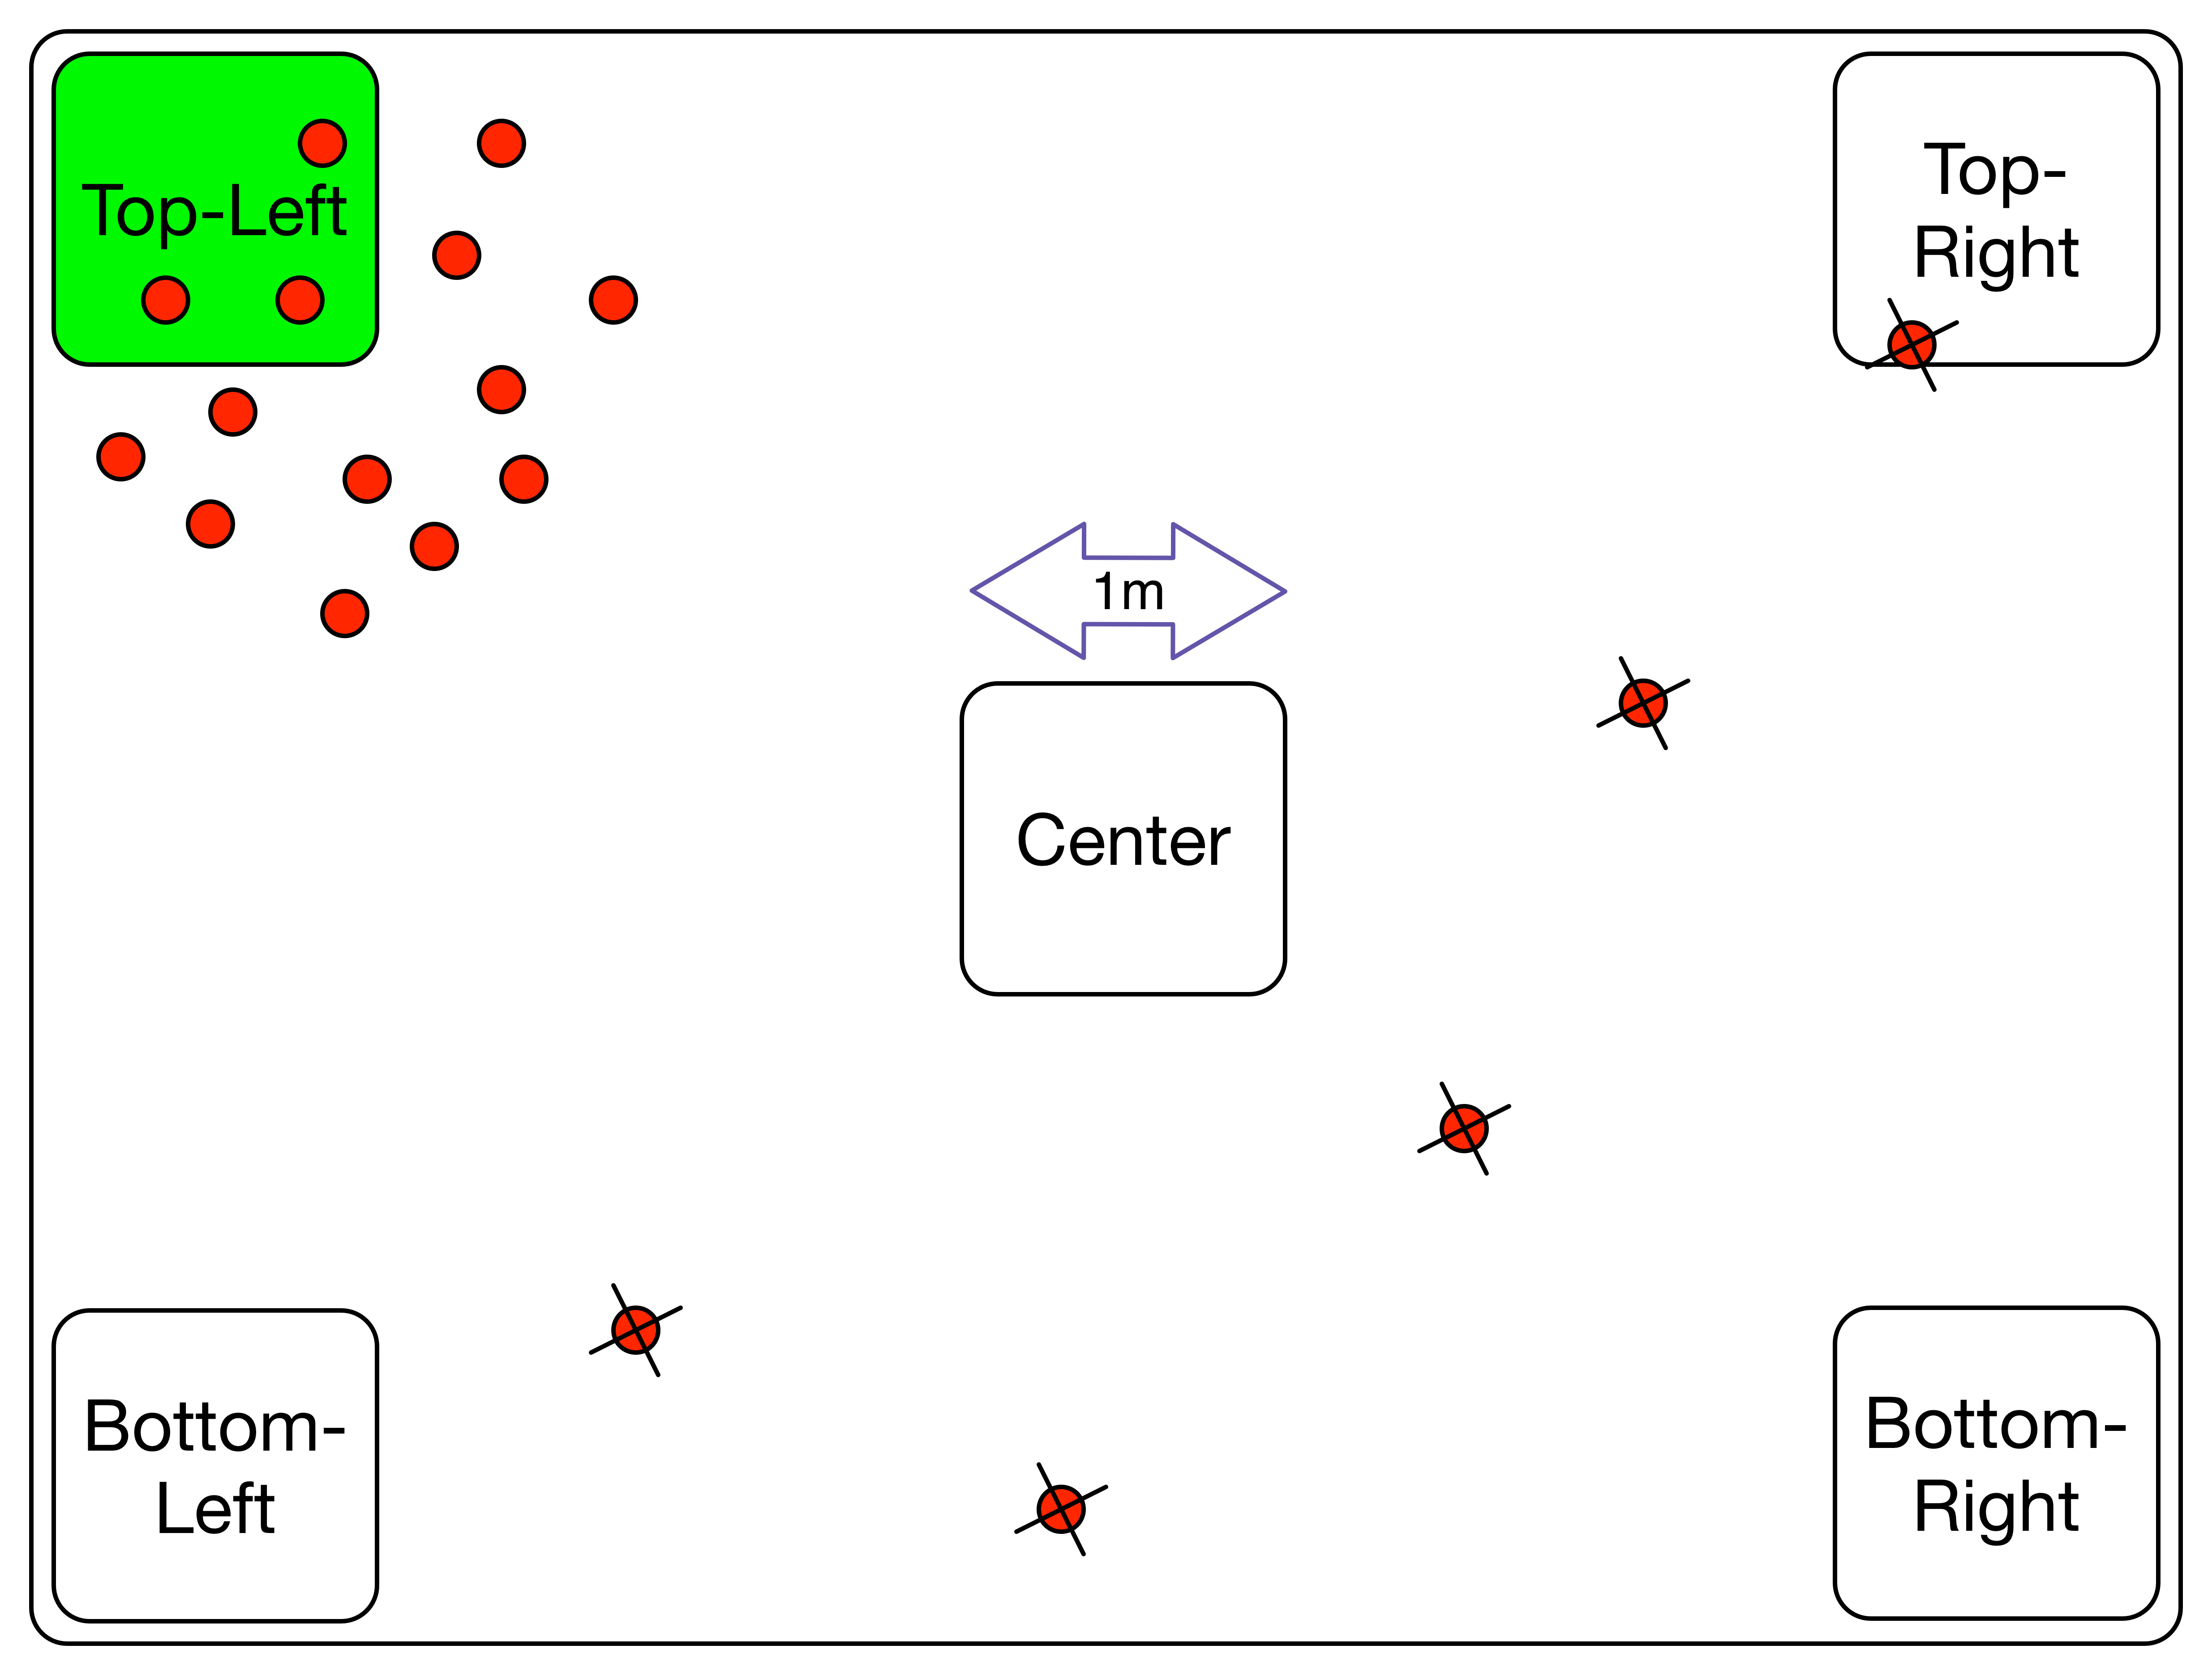
\includegraphics[width=100mm]{Figures/Landmarks.jpg}
\decoRule
\caption[Landmarks]{Five landmarks and the collection of red points predicted by the ITS.}
\label{fig:LandmarksChapter2}
\end{figure}

%----------------------------------------------------------------------------------------

\section{Reasons for Using Machine Learning}
Machine Learning is very suitable for analyzing big amounts of data. The supervised learning methods that are used in this work read the given training data and then build a model of it, which tries to distinguish the given classes. This model can then be applied to the data points collected by the user during the experiment and, in this way, it can predict the class (room or landmark respectively) of the user. By using Machine Learning methods we can take advantage of the modern smart phone's ability to collect huge amounts of data about what is happening around it.


%----------------------------------------------------------------------------------------


\section{Machine Learning Workflow}
\label{sec:MLWorkflow}

In this section we are giving a short introduction about the workflow we used to achieve the best accuracy possible for the tested datasets. We used an article about a typical machine learning workflow (\cite{ml_workflow}) as a guideline for our workflow.
%and the menu of the Weka explorer in the graphical user interface of the Weka application seen in Figure \ref{fig:WekaExplorer} 

% \begin{figure}[H]
% \centering
% 
\includegraphics[width=100mm]{Figures/WekaExplorer.jpg}
% \decoRule
% \caption[Weka Explorer]{The menu of the Weka explorer in the graphical user interface of the Weka application.}
% \label{fig:WekaExplorer}
% \end{figure}


\begin{enumerate}
\item \textbf{Data Preprocessing} \\
First, the data has to be cleaned. Redundant or insensible information has to be deleted. 
\item \textbf{Attribute Selection} \\
Second, the right attributes have to be selected. Some attributes may not contribute any useful information to the model and can therefore be discarded. Specifically for this thesis it is discussed in Section \ref{sec:AttributeSelection} and \ref{sec:AttributeExclusion}.
\item \textbf{Feature Engineering} \\
In this part of the workflow, we try to create new features, for instance in Section \ref{sec:MeanAndVariances}, or modify existing features to improve the accuracy (Section \ref{sec:Rounding}).
\item \textbf{Find Base Learners} \\
In this section, we find the best base ML method.
\item \textbf{Find Meta Learners} \\
In this step, we improve the performance using meta learners. A meta learner is defined as a combination of one or several different base learners (conventional ML algorithm). This is described in more detail in Section \ref{sec:Ensemble}.
\item \textbf{Hyper-Parameter search} \\
Finally, we use methods like autoweka, gridsearch, multisearch or trial-and-error to tweak the parameters of the chosen ML methods in order to further improve the accuracy (Section \ref{sec:HyperParameterSearch}).
\end{enumerate}

This workflow is an iterative process. In order to achieve the best results it may have to be repeated several times.


%----------------------------------------------------------------------------------------

\section{Chosen Machine Learning Algorithms}
As Weka provides a very big amount of efficiently implemented machine learning algorithms we could test lots of them without spending efforts of implementing them from scratch. An overview can be found on \url{http://wiki.pentaho.com/display/DATAMINING/Classifiers}. The following list includes the algorithms that have been implied in this thesis. Detailed information about the algorithms can be found in the method \texttt{addClassifiers()} in the class \url{https://github.com/JoelNiklaus/IndoLoc/blob/master/app/src/test/java/ch/joelniklaus/indoloc/AbstractTest.java}.

\begin{itemize}
   \item Bayes
   \begin{itemize}
     \item NaiveBayes (see \cite{John1995})
   \end{itemize}
   
   \item Functions
   \begin{itemize}
     \item LibSVM (Library for Support Vector Machines, see \cite{libsvm})
     \item Logistic (see \cite{leCessie1992})
     \item MultilayerPerceptron (Neural Network)
     \item SMO (Sequential Minimal Optimisation) (see \cite{Platt1998, Keerthi2001, Hastie1998})
   \end{itemize}
   
   \item Trees
   \begin{itemize}
     \item J48 (see \cite{Quinlan1993})
     \item RandomForest (see \cite{Breiman2001})
   \end{itemize}
   
   \item Lazy (Instance Based)
   \begin{itemize}
     \item IBk (Implementation of the K-Nearest-Neighbour Algorithm, see \cite{Aha1991})
     \item KStar (see \cite{Cleary1995})
     \item LWL (Locally Weighted Learning, see \cite{Frank2003, Atkeson1996})
   \end{itemize}
   
   \item Meta
   \begin{itemize}
     \item AdaBoostM1 (Adaptive Boosting, see \cite{Freund1996})
     \item Bagging (see \cite{Breiman1996})
     \item Dagging (see \cite{Ting1997})
     \item Decorate (see \cite{Melville2003, Melville2004})
     \item Grading (see \cite{Seewald2001})
     \item LogitBoost (see \cite{Friedman1998})
     \item RandomSubSpace (see \cite{Ho1998})
     \item Stacking (see \cite{Wolpert1992})
     \item Vote (see \cite{Kuncheva2004, Kittler1998})
   \end{itemize}
\end{itemize}

Because an explanation of all the tested algorithms would go beyond the constraints of this thesis we are giving the following recommendations for the interested reader: A good website to get an overview on \url{http://machinelearningmastery.com/a-tour-of-machine-learning-algorithms/} and a good article for more details on \url{http://alex.smola.org/drafts/thebook.pdf}.


%----------------------------------------------------------------------------------------

\section{Features}
\label{sec:Features}
In a Machine Learning project the attributes of the classes are denoted as features. Each feature is describing an aspect of the classes. In our case features are our measurements, for instance an RSS value. For the ML project to deliver a good prediction accuracy it is very important to select the right attributes/features and to also modify certain features or even create new features out of existing features. This is part of the ML workflow described in Section \ref{sec:MLWorkflow}.

In the following sections both the features used in the system and the ones taken into consideration, but then found to be useless, are introduced. Each feature corresponds to one column in the dataset and would be referred to as an attribute in Weka.

\subsection{Features used in the experiments}

In the following sections, the features which are actually used in the running system are presented.


\subsubsection{RSS}
\label{sec:RSS}
The RSS values provide the core data as they contribute the most to the performance of the ML methods. The smart phone scans the surrounding access points, obtains and registers the RSS values of each access point. These values depend on the distance to the access point as well as on the existence of obstacles, such as walls or furniture, between the access point and the device. Normally the RSS values in our datasets were between -20 and -90.

\subsubsection{Magnetic Field}
\label{sec:MagneticField}

%http://www.eecs.yorku.ca/course_archive/2014-15/W/4443/DemoPrograms/demoflat/DemoFlatActivity.html

\begin{figure}[H]
\centering
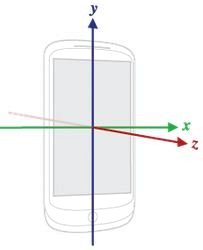
\includegraphics[width=100mm]{Figures/Device.jpg}
\decoRule
\caption[Device]{The values in the device's coordinate system.}
\label{fig:Device}
\end{figure}

\begin{figure}[H]
\centering
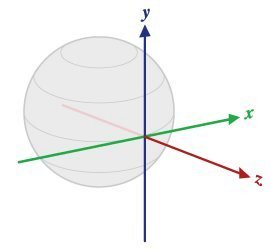
\includegraphics[width=100mm]{Figures/Earth.jpg}
\decoRule
\caption[Earth]{The values in the earth's coordinate system.}
\label{fig:Earth}
\end{figure}

The device's sensors measure the magnetic field in the device's coordinate system. As the user walks around, the orientation of the device may change all the time. We would therefore have to collect all possible values from every orientation in every point for the training phase. This would result in a huge amount of data and the training performance would be extremely inaccurate. 


In addition to the raw magnetic field values we can also derive data from the accelerometer measuring gravity in the device's coordinate system. By using the Android built in function \texttt{SensorManager.getRotationMatrix()} and providing the magnetic field and gravity values, we can get the rotation matrix \texttt{R} and the inclination matrix \texttt{I}.
Using these two matrices, we have two methods making use of the raw data (coded in \url{https://github.com/JoelNiklaus/IndoLoc/blob/master/app/src/main/java/ch/joelniklaus/indoloc/models/SensorData.java}):



\paragraph{Magnetic Processed}

With the help of \texttt{R} we then can do a change of the basis from the device's to the earth's coordinate system to get the processed magnetic values \texttt{mp}. (see \ref{magneticProcessedEq})

\begin{equation} \label{magneticProcessedEq}
\begin{pmatrix}
0 \\
mp \\
mp
\end{pmatrix} 
 = R * m
\end{equation}

Now we have got the magnetic field data at a specific point in the earth's coordinate system. The x value is in East-West Direction, the y value is in North-South Direction and the z value is perpendicular to the center of the earth. As the magnetic field of the earth only goes from one pole to the other the x value is always 0 and is therefore not used as a feature.


\paragraph{Gravity Magnitude and Geomagnetic Magintude}
In order to obtain the gravity magnitude \texttt{grm} (in z direction) we multiply the gravity vector \texttt{g} with \texttt{R}. (see \ref{gravityMagnitudeEq})


\begin{equation} \label{gravityMagnitudeEq}
\begin{pmatrix}
0 \\
0 \\
grm
\end{pmatrix} 
 = R * 
\begin{pmatrix}
g_1 \\
g_2 \\
g_3
\end{pmatrix}
\end{equation}


To obtain the geomagnetic magnitude \texttt{gem} (in y direction) we multiply the magnetic vector \texttt{m} with $I*R$. (see \ref{geomagneticMagnitudeEq})

\begin{equation} \label{geomagneticMagnitudeEq}
\begin{pmatrix}
0 \\
gem \\
0
\end{pmatrix} 
 = I * R * 
\begin{pmatrix}
m_1 \\
m_2 \\
m_3
\end{pmatrix}
\end{equation}

\paragraph{Additional information}
In order to reduce extreme variations which might disturb the ML algorithms, we apply a low-pass-filter to the newly collected data. For the alpha value we chose 0.75. So the last value has a weight of 0.75 and the newly collected value a weight of 0.25.
The accuracy of the magnetic field sensor in the devices we tested is 0.15 \textmu T. But still the data the sensor outputs contains many more decimal places. In order to exclude the noise, we round the values to 1 \textmu T. 
The values obtained by measuring the magnetic field provide an improvement to the overall accuracy.



\subsubsection{Light}
We also thought about including data collected from the light sensor because, for instance, a room facing a window will clearly be brighter than one surrounded by walls only. As can be seen in Section \ref{AdditionalFeatures} this does improve the prediction accuracy, however, these assumptions are not stable over time. In the night, there may be no difference concerning light at all between the two previously mentioned rooms. Or if there is a cloudy day the overall light strength would probably be much less as compared to that on a sunny day. Thus, it might be appropriate to work with light differences to a representative data point. This data point would have to be chosen carefully and would have to be recorded first. 

We include this suggestion here because it improves the result but it still has to be tested if it is worth integrating it into a system in a productive environment.


\subsection{Non-useful features}
In the following sections the features which have been taken into account but have been judged as not helpful are presented. These features are therefore not included into the running system, as they would only produce additional overhead and slow down the generation and evaluation of the ML models.

\subsubsection{Ambient temperature}
At first we thought about including the ambient temperature as another feature because there may be characteristic small temperature differences between rooms which could help in making predictions.

However, we estimate this feature to be rather unpredictable. For instance when someone turned the heating up in one specific room, the temperature would change drastically. As a consequence, we would suddenly receive incredibly conflicting values. Or imagine someone opens the window on a very cold day. Even without any human interference, different seasons or poor isolation of walls or windows could have an influence on temperatures in the same room.
Apart from that, there are still lots of devices which do not yet have any temperature sensors.

\subsubsection{Relative Humidity}
Another idea would have been to include relative humidity. In comparing a bathroom and an office, for instance, it would be a fair assumption that the relative humidity would be higher in the former than the latter.
But, as with the ambient temperature, we think that it is too volatile overall. An open window on a rainy day or even just a hot steaming tea can change the humidity landscape of a room. And here as well, there are not many devices which already have a relative humidity sensor built in.


\subsubsection{Pressure}
Relative pressure differences are utilized in the ITS to distinguish between different floors of a building. But this work is only part of the ITS and only has to provide predictions on the same floor. Therefore, it does not make sense to include it in this system. Furthermore, the Motorola test device was not even equipped with a pressure sensor.

\subsubsection{Mean and Variances of RSS}
\label{sec:MeanAndVariances}
One idea was to include the mean and the variances of the RSS values. But as experiments have been able to show, this does not improve the overall accuracy. This is probably the case because it does not add additional information to the ML algorithms but just alters and adds pre-existing ones.


\subsubsection{GPS}
An idea is to include the latitude and longitude gained from the GPS to help prediction close to the windows. But as our tests in Section \ref{AdditionalFeatures} have shown the accuracy is decreased if it is included.


%----------------------------------------------------------------------------------------

\section{Weka}
Weka, standing for Waikato Environment for Knowledge Analysis, is an open source machine learning library programmed in Java developed by the University of Waikato, New Zealand, and can be found on \url{http://www.cs.waikato.ac.nz/~ml/weka/}.

Two reduced versions for Android \footnote{rjmarsan: \url{https://github.com/rjmarsan/Weka-for-Android}} \footnote{Shookit: \url{https://github.com/Shookit/android-ml-weka}} have been considered and the first version (from the developer with user name rjmarsan) has been chosen. It uses Weka 3.7.3 and mainly does not include the GUI (Graphical User Interface) parts of the system which are not used in this application.

\subsection{Advantages}
The main reason why we chose the library Weka, is the huge amount of efficiently implemented ML algorithms it provides. It offers a wide range of both supervised and unsupervised learning algorithms. Furthermore, in addition to the Java interface there is both a command line interface and a graphical user interface available.

\subsection{Disadvantages}
Although the introduction documentation \footnote{Programmatic Use: \url{https://weka.wikispaces.com/Programmatic+Use}} \footnote{Weka in Java Code: \url{https://weka.wikispaces.com/Use+WEKA+in+your+Java+code}} provides you with some information to get started, the Javadoc \footnote{Javadoc: \url{http://weka.sourceforge.net/doc.stable/}} is not of much use. It only provides one very small sentence to most of the methods (functions). This sentence mostly does not add any additional details to the information from the method's name. 

The Javadoc for the classes is slightly better though, providing some explanation how to use it. The design of the methods is very close to the use of the command line. So usually a string array of cryptic options has to be provided in order to configure the classifier. Sometimes it can be done using setter methods, but if so it is poorly documented what exactly is altered by setting a certain value.

There is a mailing list \footnote{Mailing List: \url{https://list.waikato.ac.nz/mailman/listinfo/wekalist}} and a forum on Pentaho \footnote{Pentaho Forum: \url{http://wiki.pentaho.com/display/DATAMINING/Pentaho+Data+Mining+Community+Documentation}} where questions concerning Weka can be asked. But unfortunately the active community does not seem to be very large. For my problems at least, we had great difficulties finding answers through these two channels.


%----------------------------------------------------------------------------------------


\section{Android App}

\subsection{Implementation}
If the reader is interested in knowing how to implement an Android app we can recommend the following web resources: Android Developers on \url{https://developer.android.com/index.html} and Android Studio on
\url{https://developer.android.com/studio/index.html}.



\subsection{Reasons for Choosing the Android System}
The most important reason which lead to the choice of Android as a (first) platform of the app was the ITS which is being implemented in Android. On top of that, Weka offers a Java interface which makes it very easy to integrate into an Android app.

\subsection{Tested Mobile Phones}

First, we tested the Android app on the Emulator in Android Studio. This was fine for examining how the user interface behaved but after we added the WiFi, Sensor and GPS collection, we had to test it on real phones. We used the following two Android phones:
Nexus 4 (LG, Android Version 5.0, API, Level 22, Accurate Specifications on  \url{https://en.wikipedia.org/wiki/Nexus_4}) and Moto X Style (Motorola, Android Version 6.0, API Level 24, Accurate Specifications on  \url{https://www.digitec.ch/en/s1/product/motorola-moto-x-style-570-32gb-21mp-black-mobile-phones-5339851}).
%----------------------------------------------------------------------------------------




 
% Chapter 3

\chapter{Implementation and Experimentation} % Main chapter title
\label{Chapter3} % For referencing the chapter elsewhere, use \ref{Chapter3} 


%----------------------------------------------------------------------------------------

In this chapter, the experiments and their setup are explained. Further, we present the datasets which are used in the experiments.

\section{General Remarks}The larger the physical gap between rooms or landmarks respectively, the larger are the differences in the measured features. As a consequence, the space between the different classes in the hyperspace is increased, which makes it easier for the ML algorithm to distinguish between the classes.

%----------------------------------------------------------------------------------------
\section{Implementation}
This section gives some details about how to use Weka as open source ML library to make the predictions of rooms or landmarks respectively. Figure \ref{fig:Architecture} shows the dataflow and the different components of the Android app in a visualized way. Sensor and RSS values are measured by the device and received in the Android app. This data is then passed to a Weka component, which trains the ML algorithms. The trained algorithms are then evaluated with test data to find the one with the highest prediction accuracy. Finally, the best trained ML algorithm is then used for live testing finally returning the device's location.

\begin{figure}[H]
\centering
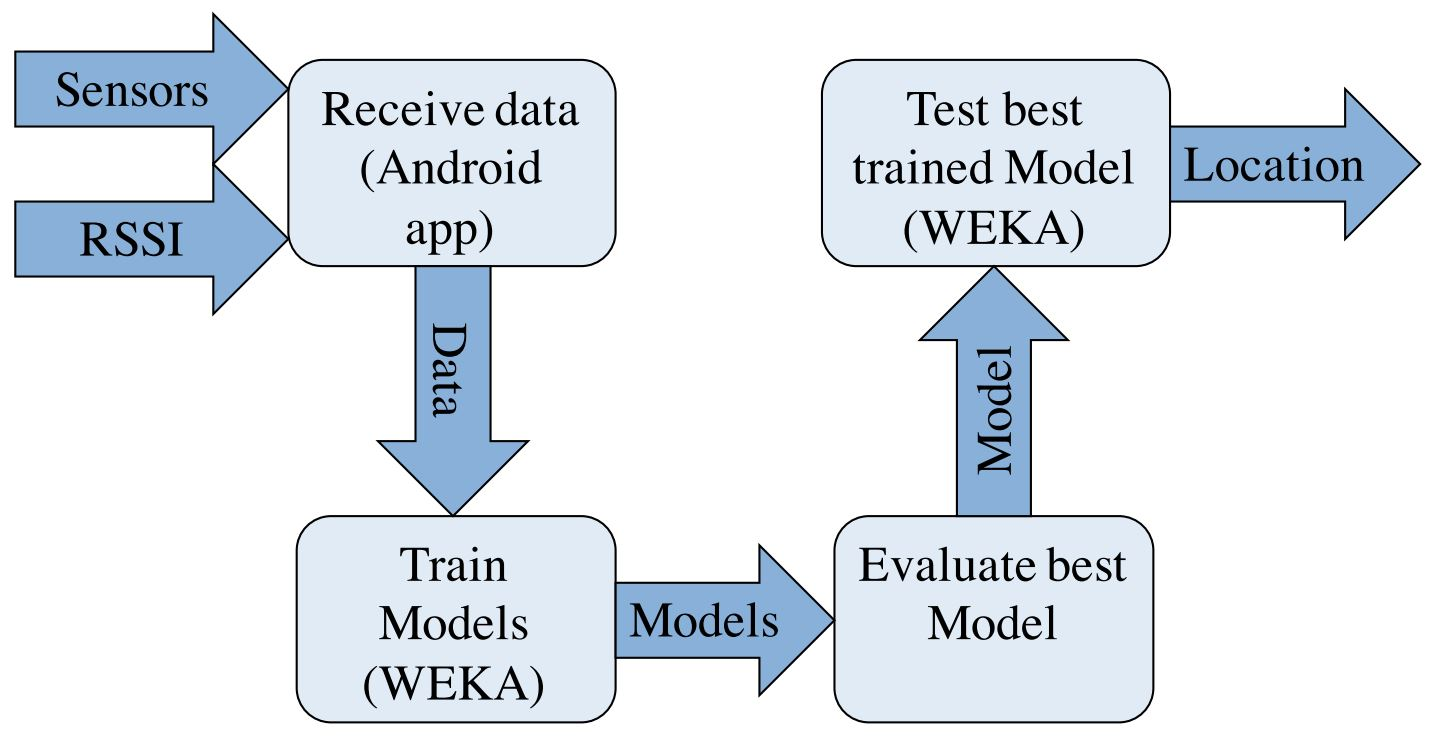
\includegraphics[width=100mm]{Figures/Architecture.jpg}
\decoRule
\caption[Architecture]{The architecture of the implemented android app.}
\label{fig:Architecture}
\end{figure}

%----------------------------------------------------------------------------------------
\section{Machine Learning Applications}

\subsection{Room Recognition}
In the room recognition phase we want the system to distinguish several rooms on the same floor. As mentioned above, the sensor accuracies are not high enough to enable the ability to distinguish data points collected at the border of two rooms. Our best practice was leaving one square metre of space at the doors without any data points collected.


\subsection{Landmark Recognition}
In the landmark recognition phase we want the system to distinguish several landmarks inside the room. As explained before, a landmark is defined as a small area within a room. Typically a landmark was of one square metre size and between each of the landmarks we left at least 2 metres space. This was our best practice and there may be better ways to do this. So in a small room (around 3x3 metres) we would have two landmarks, so one at each end. In a normal office-sized room (around 5x5 metres) we would have four landmarks, one in each corner. In a big room (around 7x7 metres) we would have five landmarks, one in each corner and one in the centre. In our experimental environment there were no bigger rooms available. (Figure \ref{fig:LandmarksChapter3})

\begin{figure}[H]
\centering
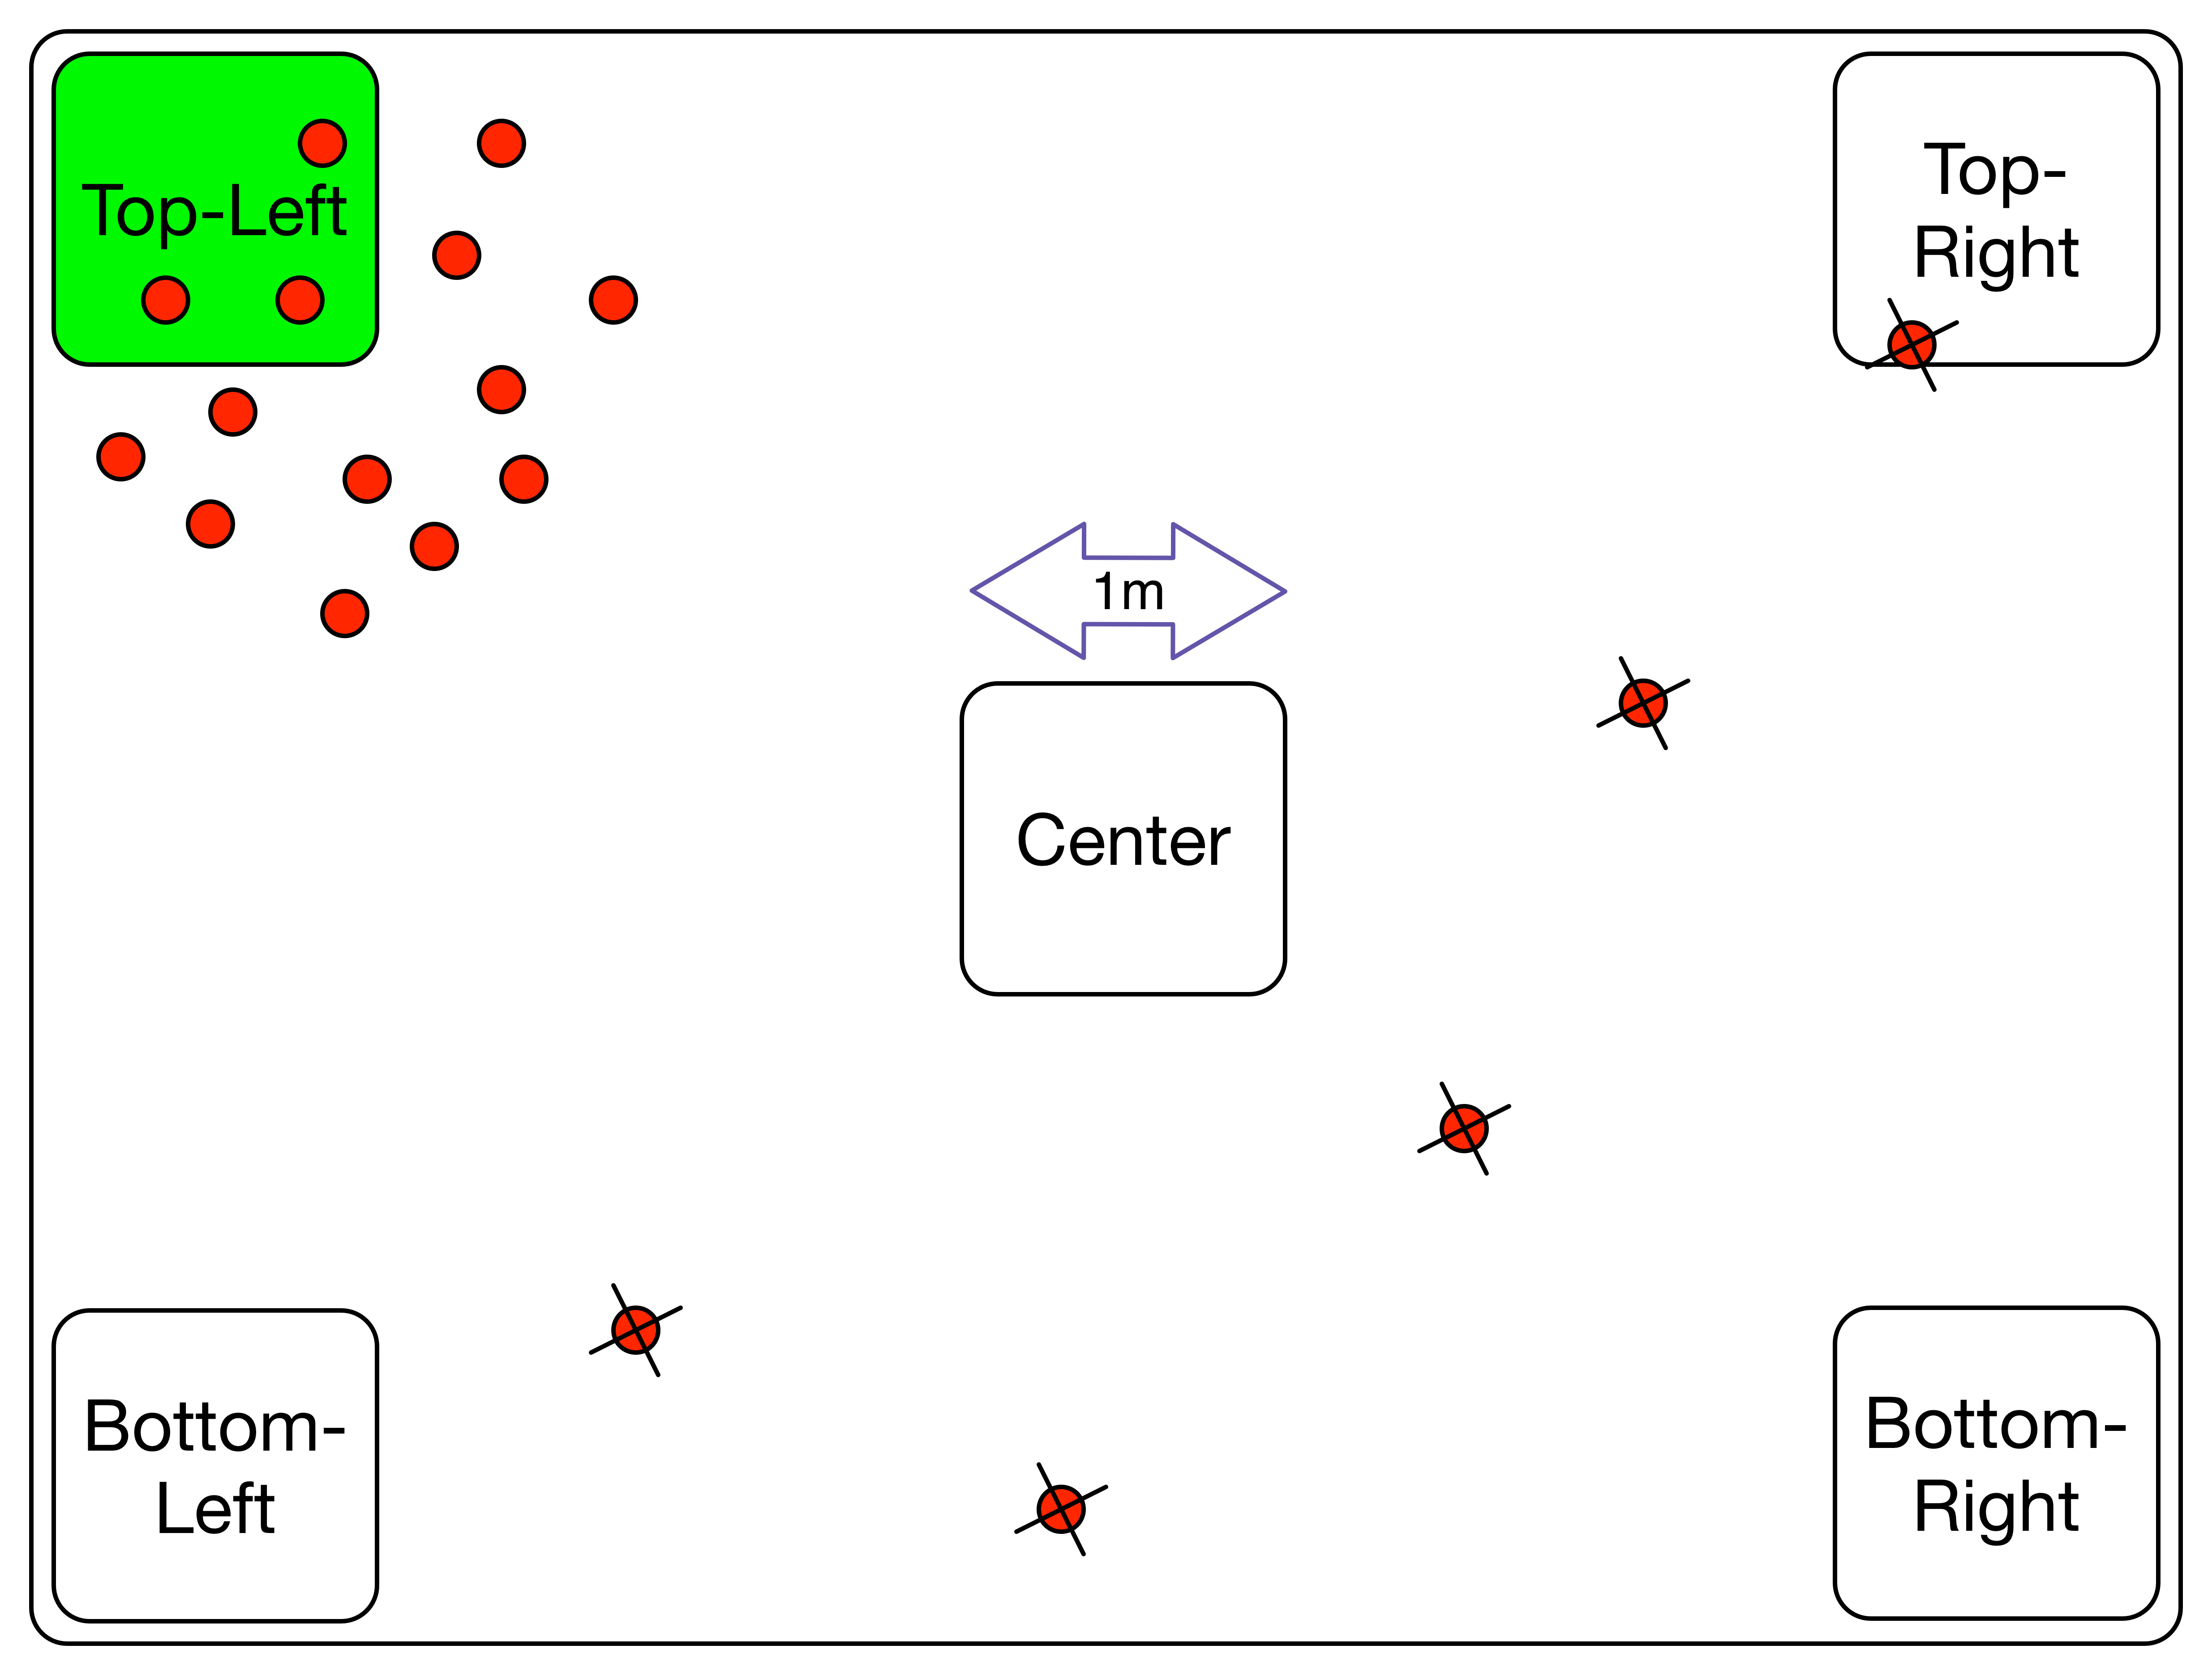
\includegraphics[width=100mm]{Figures/Landmarks.jpg}
\decoRule
\caption[Landmarks]{Five landmarks and the collection of red points predicted by the ITS.}
\label{fig:LandmarksChapter3}
\end{figure}


%----------------------------------------------------------------------------------------

\section{Data Collection Methodology}
\label{sec:DataCollection}

\begin{figure}[H]
\centering
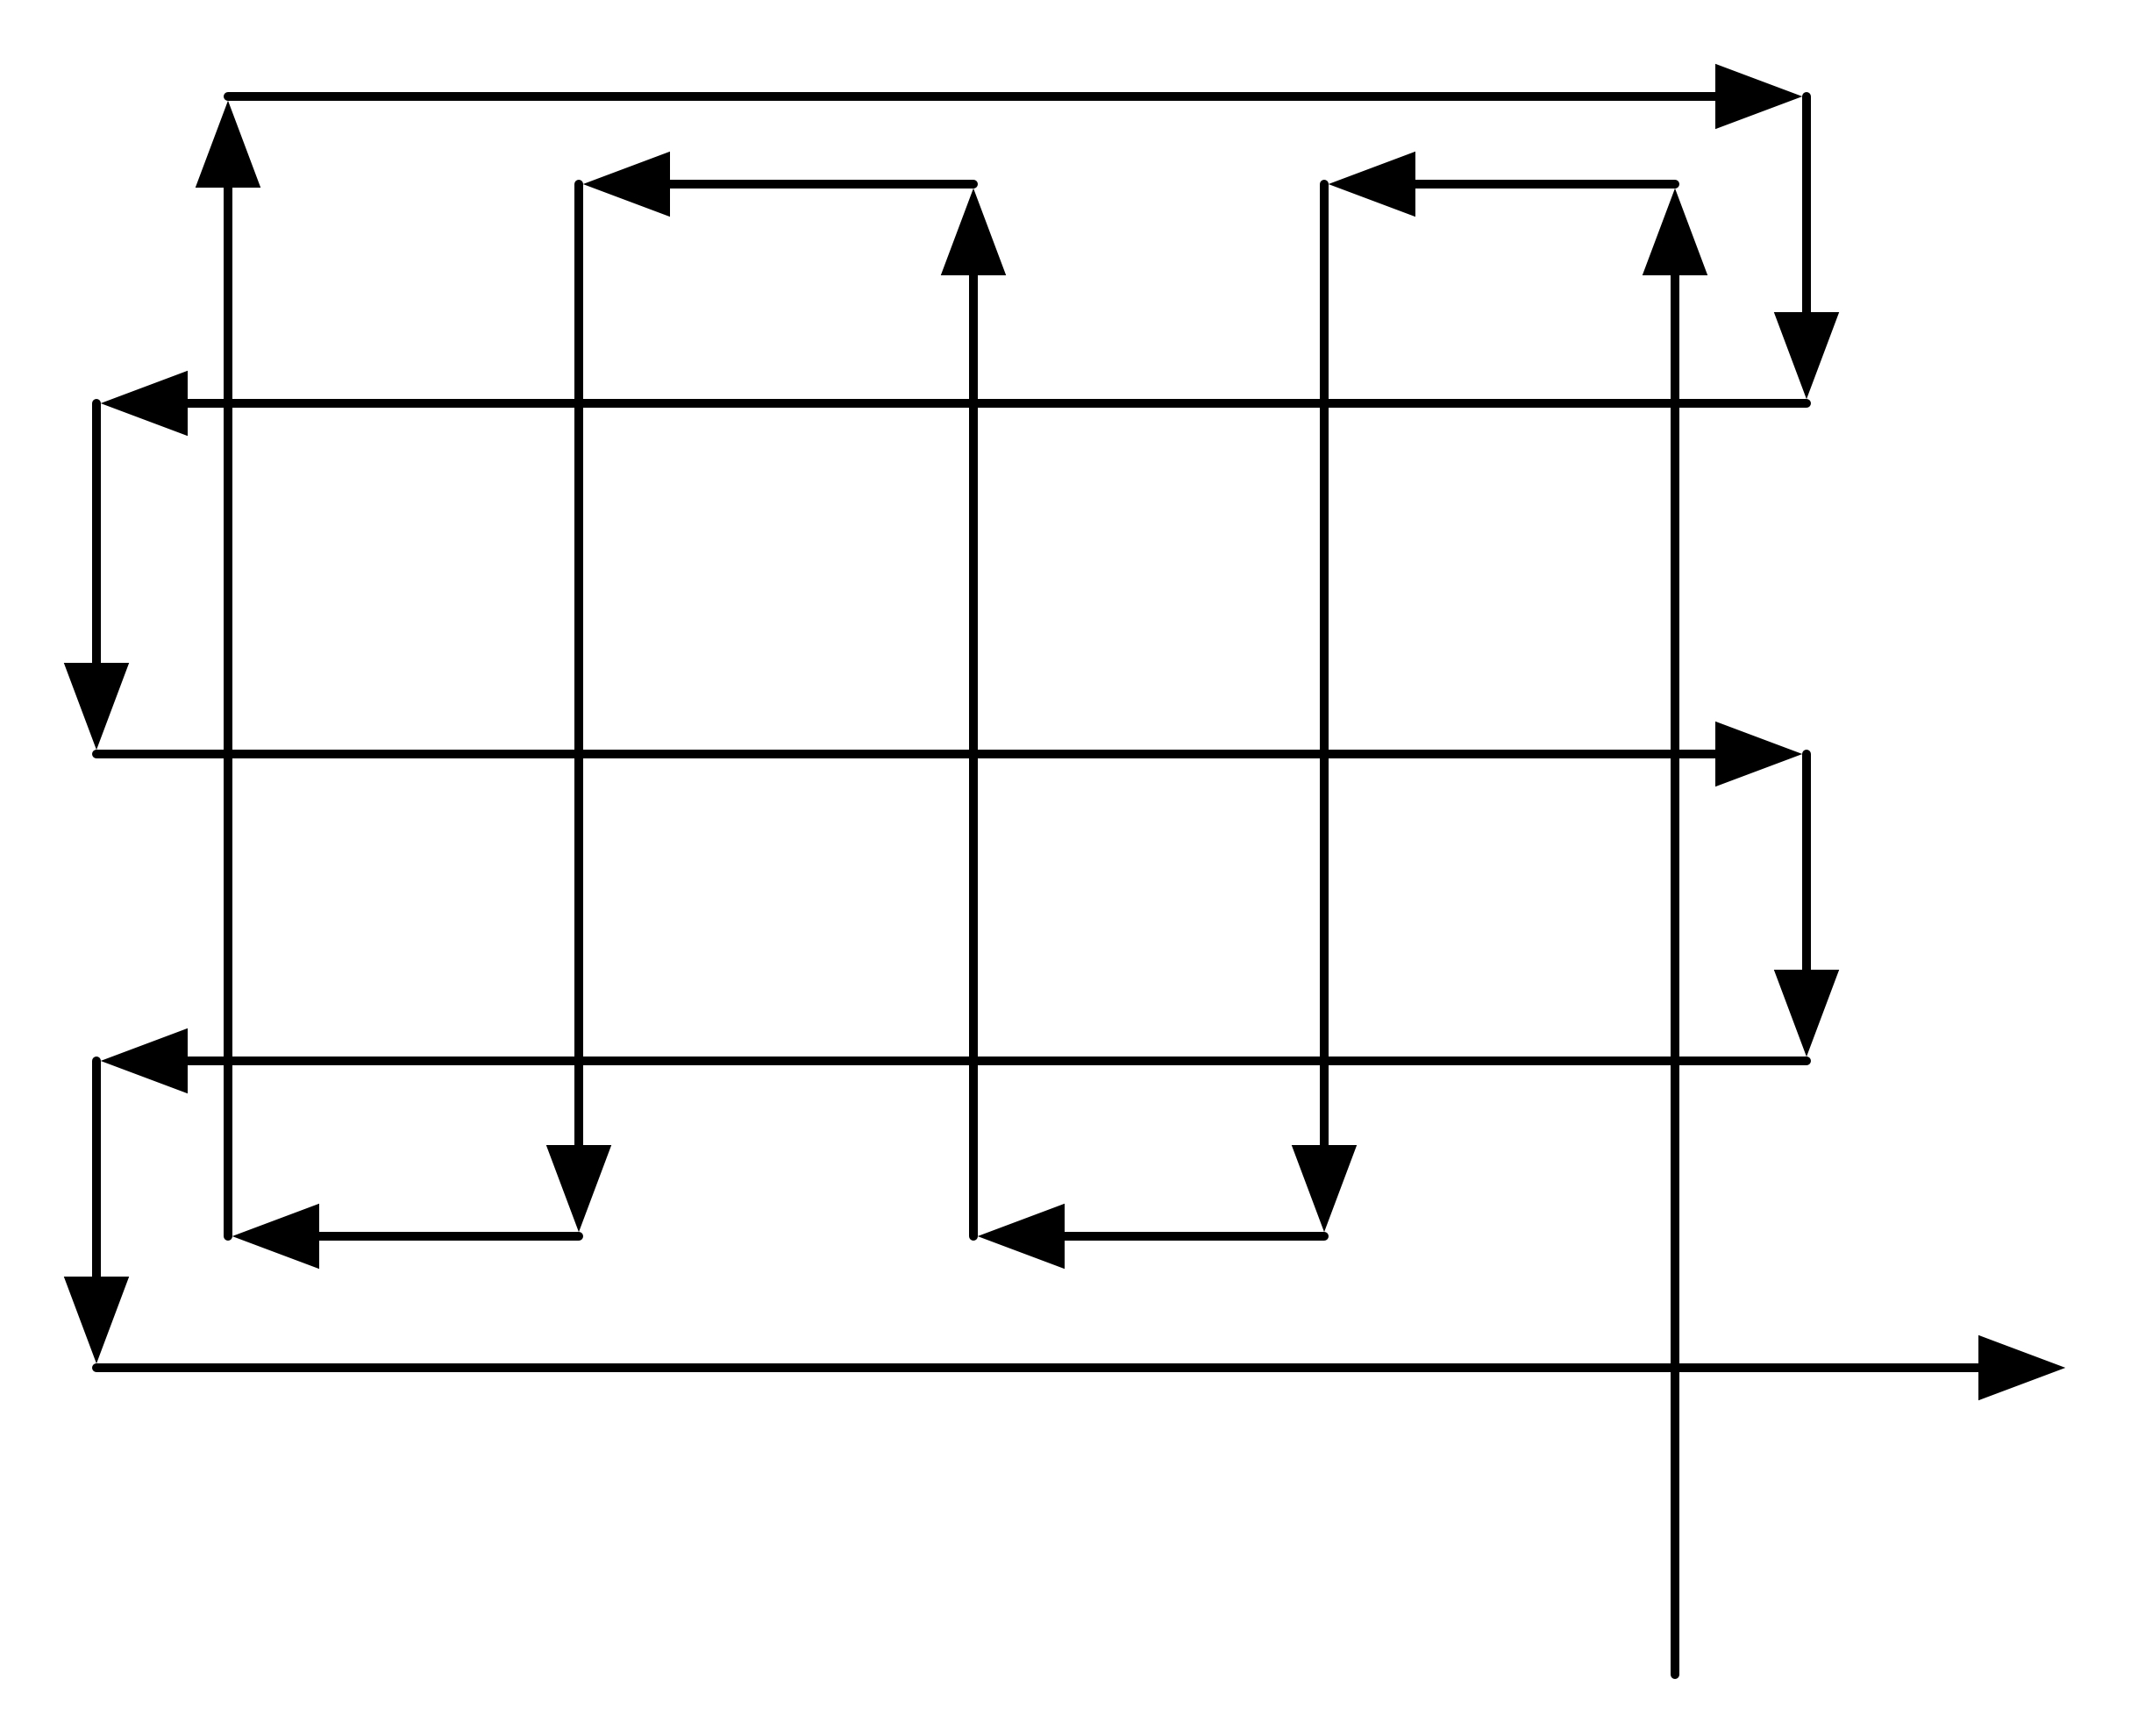
\includegraphics[width=100mm]{Figures/Grid.jpg}
\decoRule
\caption[Grid]{The grid pattern used to collect the data points.}
\label{fig:Grid}
\end{figure}
The data collection for both the training set and the test set have been done in a grid pattern, as shown in Figure \ref{fig:Grid}. So we started with the phone in one corner of the room or landmark respectively. Then, we continuously moved the phone back and forth in parallel vertical lines. Once we covered the entire area in vertical lines, we turned the device by 90 degrees and did the same in parallel horizontal lines until we arrived at the diagonally opposing corner. The distance between these lines was typically around 5cm. Using this grid pattern method, a very tightly woven net could be laid across the area. Therefore, the diversity of the collected data points could be maximized. Additionally, this way of collection data is very fast. For instance, it takes 20 minutes to finish the entire data collection in the third floor of institute building in Bern.

The training set and the testing set have been collected in two different gatherings within two hours on the same day. Because when they were collected in the same gathering and split up afterwards, Random Forest normally had over 99\% testing set accuracy in offline testing on the computer. But in live testing on the smart phone this accuracy was nowhere close (< 70\%). %The interested reader can see further information in the \href{https://github.com/JoelNiklaus/IndoLoc/blob/master/app/src/test/java/ch/joelniklaus/indoloc/experiments/OneDatasetTest.java}{One Dataset Test}  in my repository.

\begin{figure}[H]
\centering
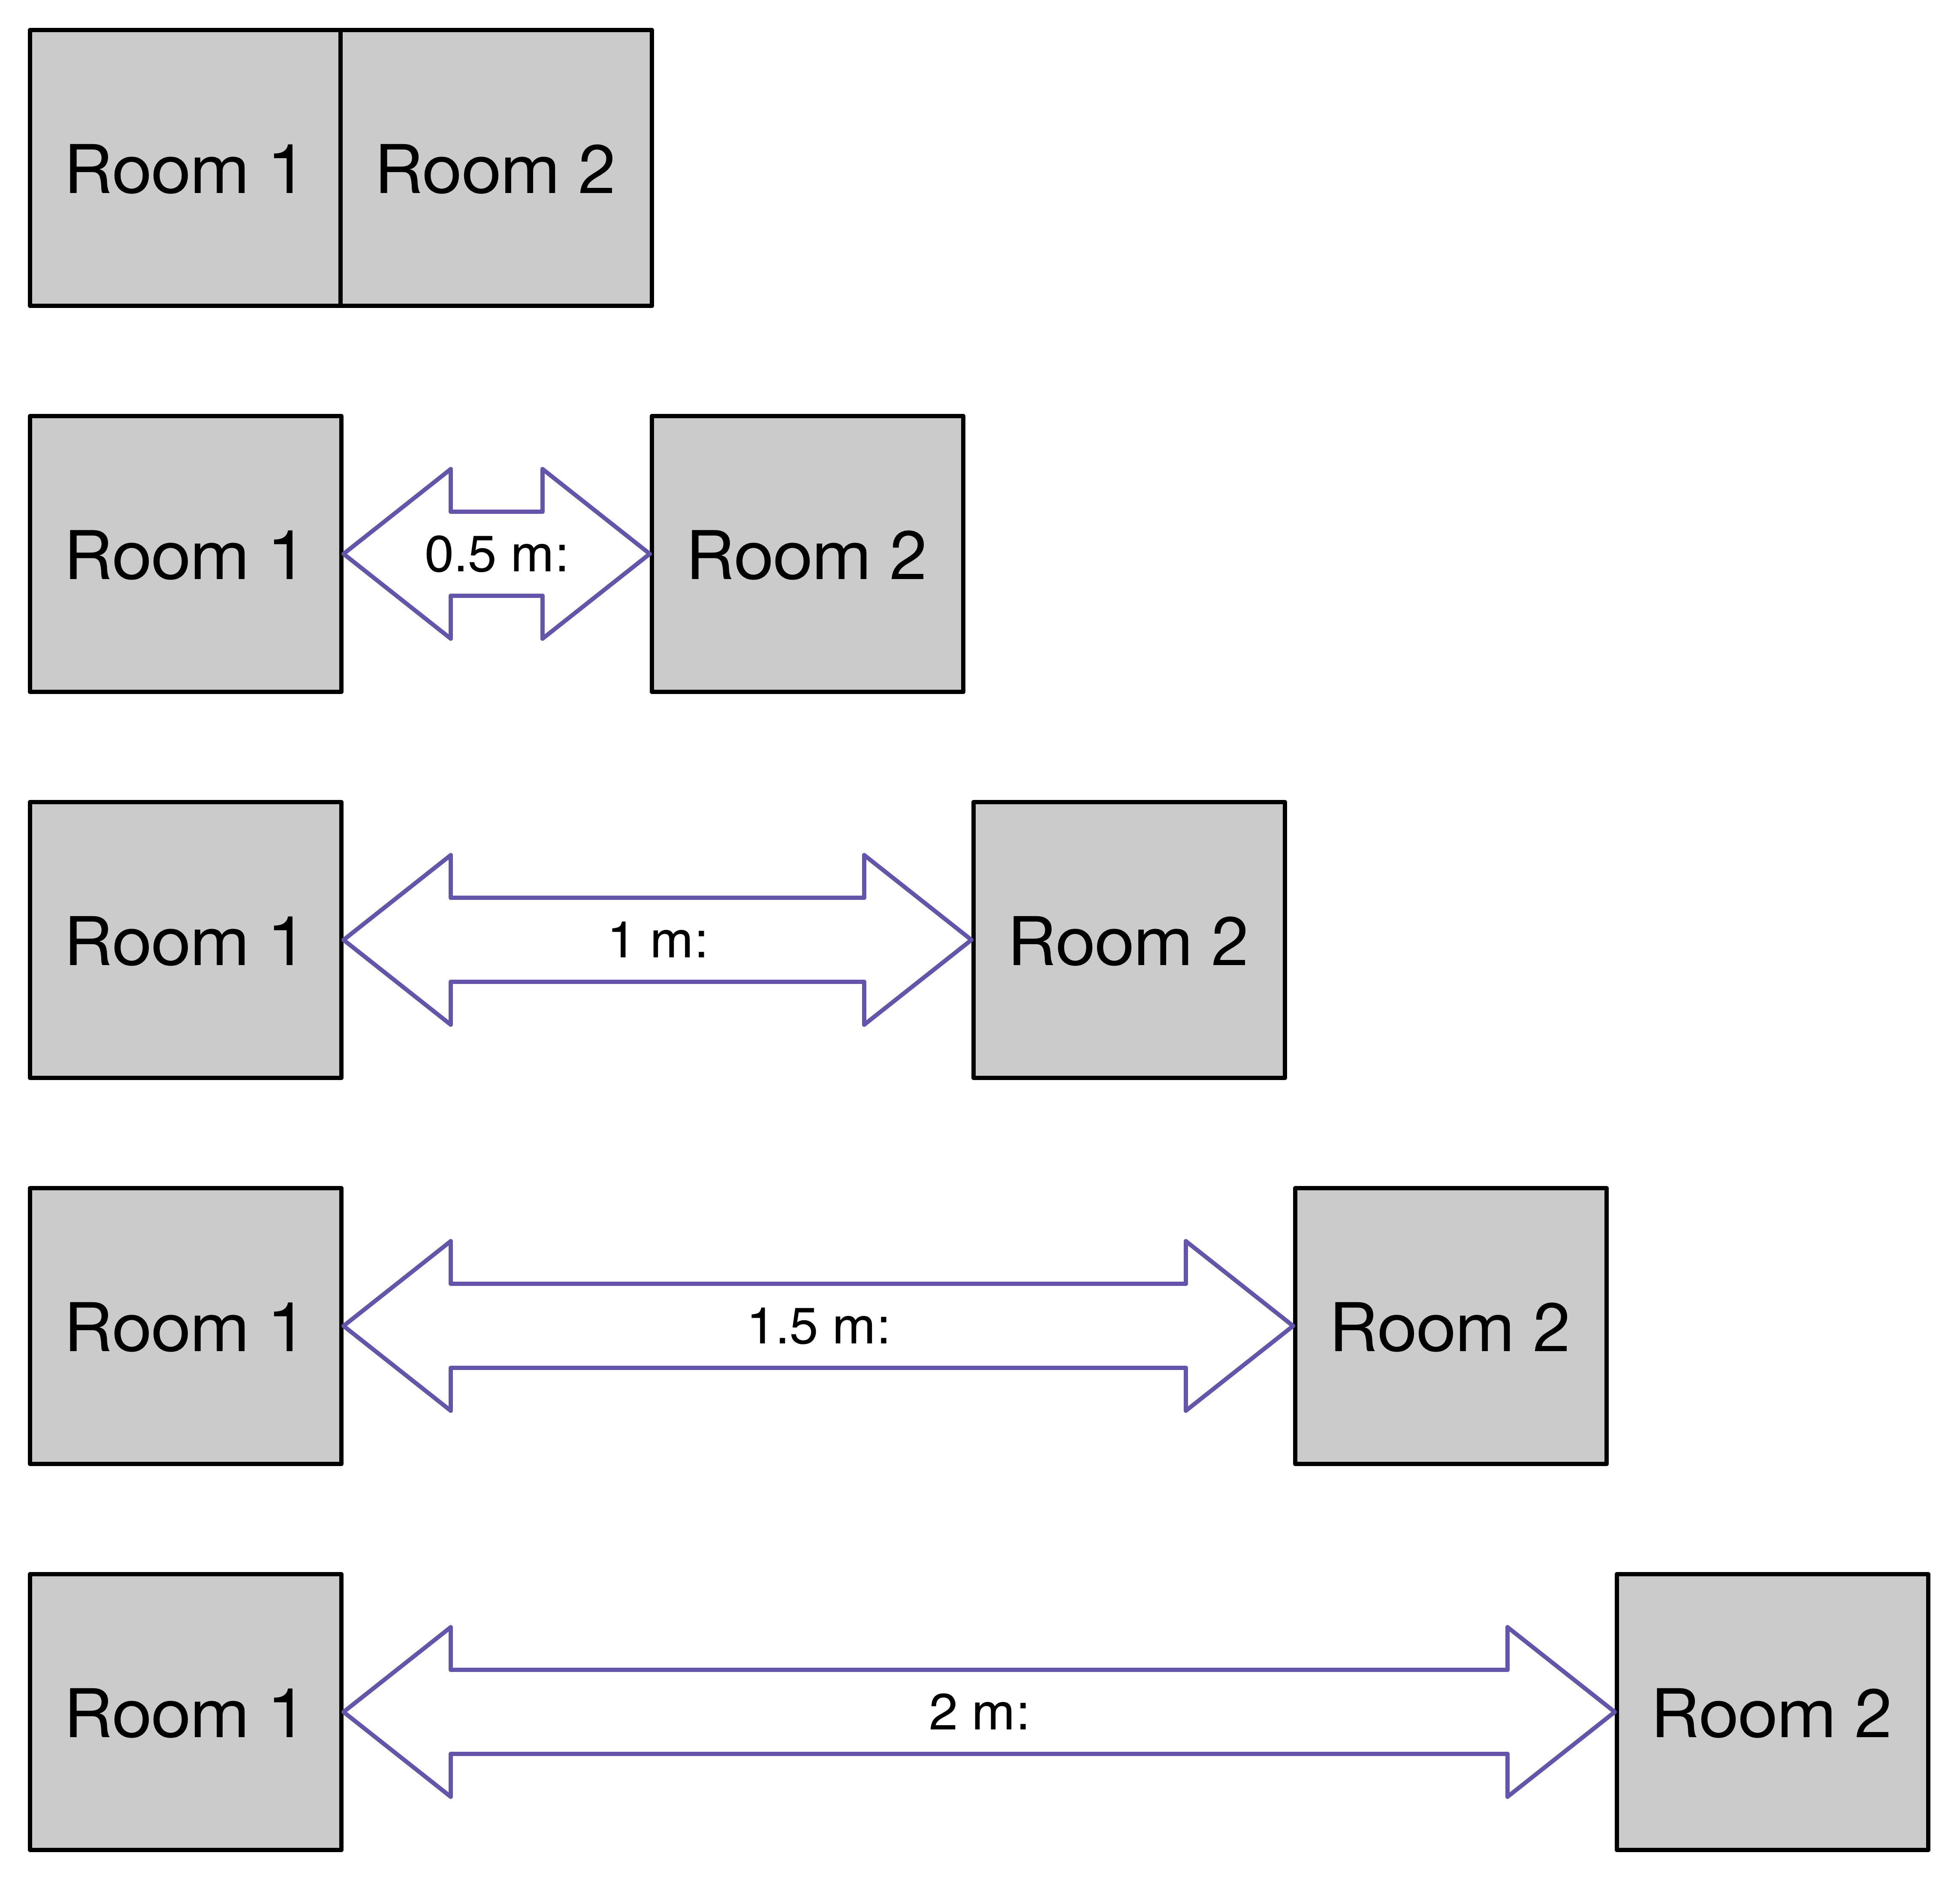
\includegraphics[width=100mm]{Figures/Distance.jpg}
\decoRule
\caption[Distance]{Distance between rooms.}
\label{fig:Distance}
\end{figure}

In supervised ML projects a class denotes the prediction output of the given ML algorithm. In our room prediction case the classes would be the different rooms and in analogy in our landmark prediction case the classes would be the different landmarks.

Generally, the physically closer together the classes are, the lower is the accuracy of the algorithms. This is due to small differences in the measured values (as shown in Figure \ref{fig:Distance}).

So on the one hand, when the distance between the classes is large, the measured values have greater differences between each other. This makes it easier to distinguish the classes and results in a higher prediction accuracy. However, this prediction is also less useful because there is a big uncategorized space in between the classes (as shown in the bottom row in Figure \ref{fig:Distance}).

On the other hand, if the distance between the classes is small, the measured values have smaller differences between each other. This of course exacerbates the problem of distinguishing the classes as the data points close to the border but in different classes have very similar values. But this prediction is much more helpful since more of the space can be categorized into a class (as shown in the top row in Figure \ref{fig:Distance}).
%But here we have to be careful, because if the prediction accuracy is not high enough we can assume that a high percentage of the mistakes the prediction makes are close to the border. 

So we have to find an optimal solution in between the two above extremes, which gives us a good accuracy but also does not come with too much uncategorized space.  Gathering from our experience we need an approximate distance of 1.5 metres between different classes to achieve an prediction accuracy of 85\%. 


In the method \texttt{registerListeners()} in the Sensor Helper class (on \url{https://github.com/JoelNiklaus/IndoLoc/blob/master/app/src/main/java/ch/joelniklaus/indoloc/helpers/SensorHelper.java}) we set the collection delay to \texttt{SENSOR\_DELAY\_NORMAL}. Looking at the Android Documentation (on \url{https://developer.android.com/guide/topics/sensors/sensors_overview.html}) we read that this delay is set to 200000 microseconds. Therefore, the sensor returns at least (!) 5 values per second.
% The WiFi collection rate is lower than the ones for the sensors.
So we collected around 5 data points per second walking at a constant rate.



%----------------------------------------------------------------------------------------
\section{Datasets}

A dataset consists of two separately collected subsets, the training and the test set. The training set usually is larger than the test set. Normally we use splits like 70\% training set and 30\% test set or 80\% and 20\%.

\subsection{Bern Dataset}
\label{sec:BernDataset}
The dataset considered for room recognition has been recorded on the third floor of the Computer Science building of the University of Bern at Neubrückstrasse 10, as shown in Figure \ref{fig:Bern}. It can be found on the github repository on \url{https://github.com/JoelNiklaus/IndoLoc/tree/master/app/src/main/assets/thesis/bern/room}.

\begin{figure}[H]
\centering
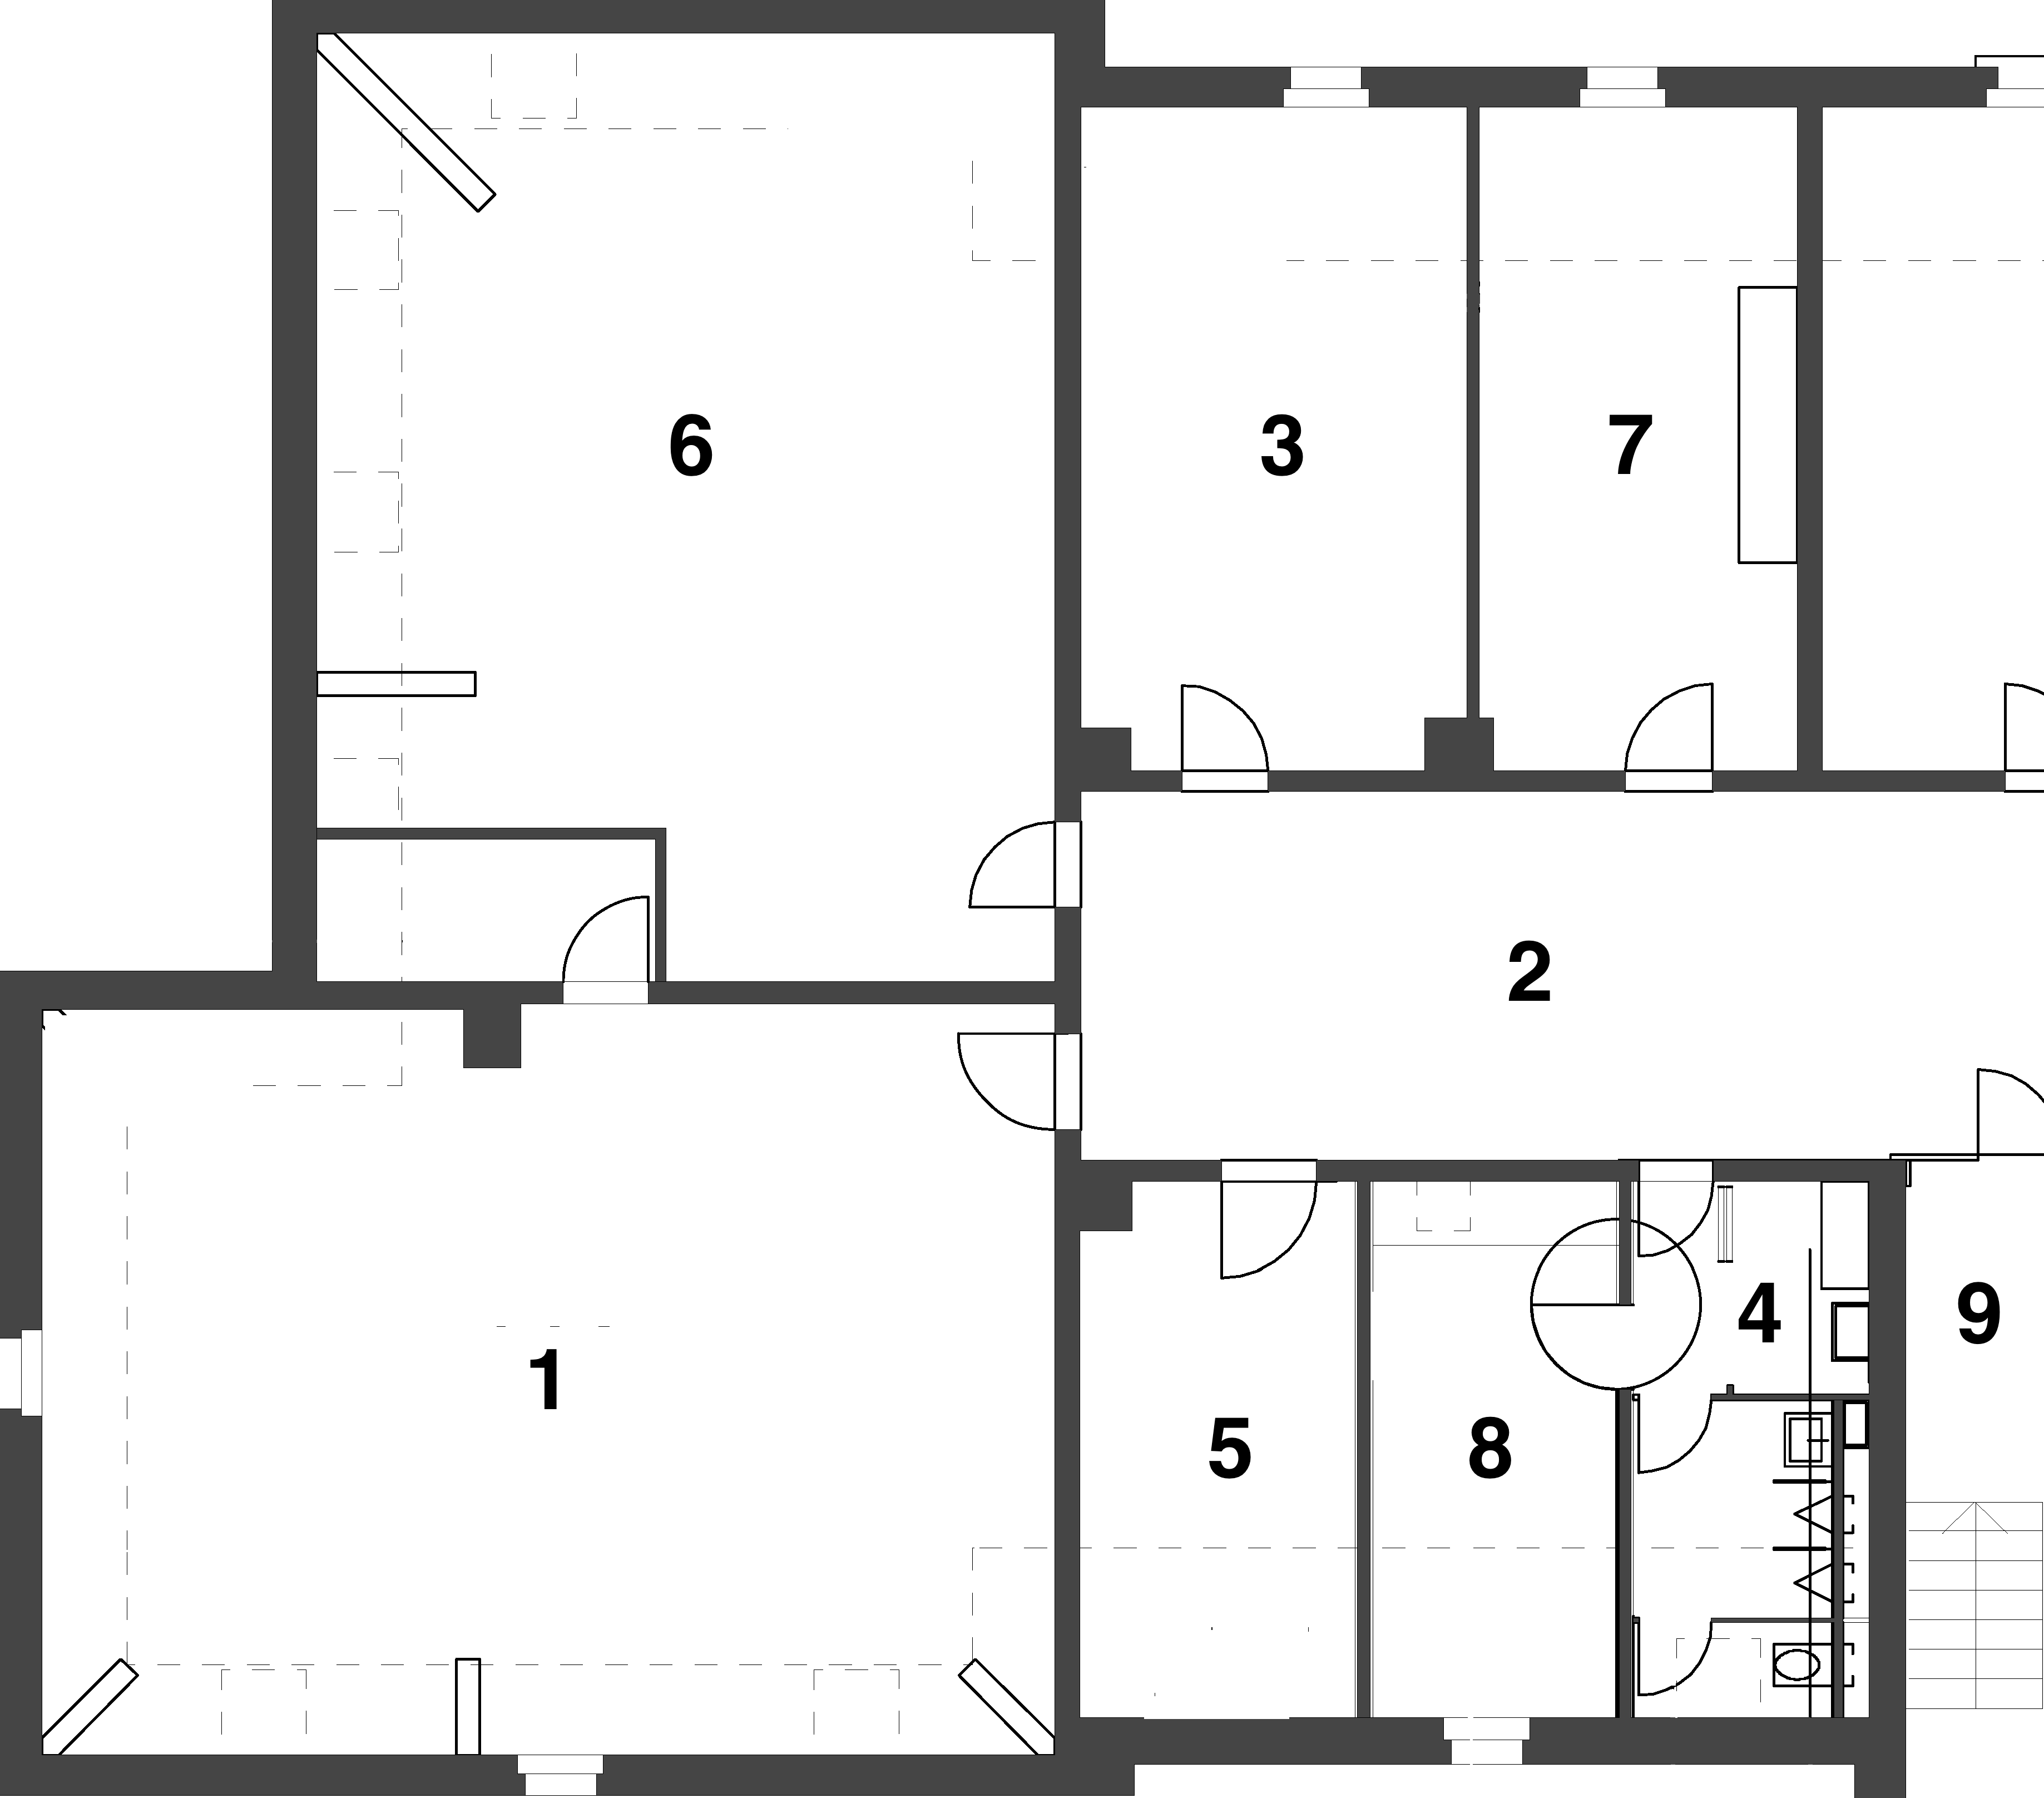
\includegraphics[width=100mm]{Figures/Bern.jpg}
\decoRule
\caption[Bern]{The testing environment in Bern.}
\label{fig:Bern}
\end{figure}

The training set contains 14569 data points in total. 3061 data points were collected in the biggest room (1) and 514 in the smallest room (4). As mentioned in Section \ref{sec:DataCollection} around 5 data points can be collected per second. Therefore, collecting the whole training set required around 50 minutes.

The test set contains 8624 data points with 2164 in room 1 and 291 in room 4. Collecting the whole test set required around 30 minutes.
In this dataset we collected all the features described above. So, in this section it is also described which of the features improve the accuracy and which of them could be left out.

This dataset is used to conduct experiments on room recognition level and on which features are beneficial for accuracy.

\subsection{Exeter Dataset}
\label{sec:ExeterDataset}
The dataset considered for landmark recognition has been recorded on the first floor of the living room in Block C in James Owen Court on Sidwell Street in Exeter, an apartment complex owned by the University of Exeter, as shown in Figure \ref{fig:Exeter}. It can be found on the github repository on \url{https://github.com/JoelNiklaus/IndoLoc/tree/master/app/src/main/assets/thesis/exeter/landmark}.

\begin{figure}[H]
\centering
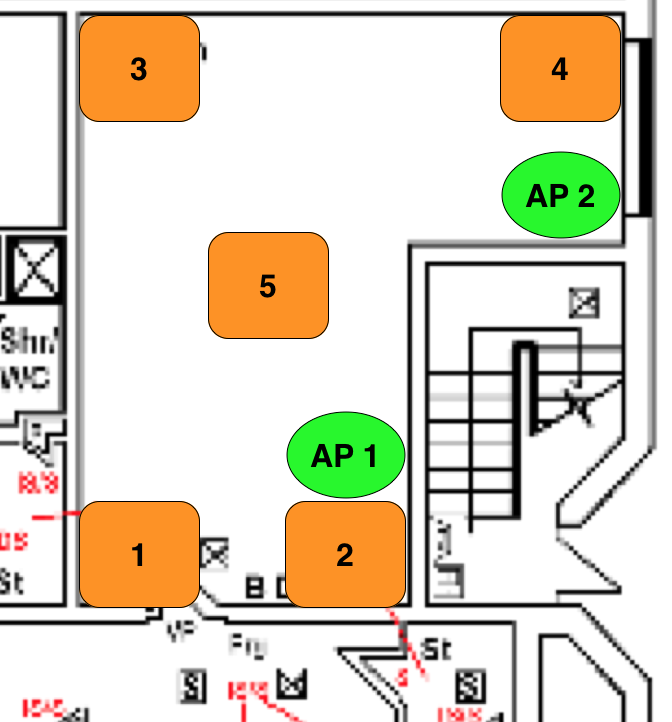
\includegraphics[width=100mm]{Figures/Exeter.jpg}
\decoRule
\caption[Exeter]{The testing environment in Exeter.}
\label{fig:Exeter}
\end{figure}



The training set contains 2522 data points in total. As each of the landmarks are of equal size we collected a little over 500 data points in each of them. Collecting the whole training set required approximately 10 minutes.

The test set consists of 1269 data points with a little over 250 data points in each landmark. Collecting the whole test set required approximately 5 minutes.

In this dataset we only collected the magnetic field values in the y and z directions, and the RSS values, because at the time of collection we presumed these to be important features. There are many different machine learning methods and they can each be parametrized in a variety of ways. Furthermore, each feature combination can be tested if it improves the result. So, in the following sections we am confining ourselves to the most expressive findings.

This dataset is used to conduct experiments on the landmark recognition level and to check if removing duplicates improves the result (\ref{sec:DuplicatesRemoval}).

%COMPARE WITH LANDMARK CDS!!

In every section there is a link available at the top which leads directly to the Java class doing the described experiment.


% Chapter 4

\chapter{Experimental Results} % Main chapter title
\label{Chapter4} % For referencing the chapter elsewhere, use \ref{Chapter4} 


%----------------------------------------------------------------------------------------

This chapter describes the results of the experiments. 
%I have made the experience that the accuracy reached depends greatly on the environment. 
On the github repository (\url{https://github.com/JoelNiklaus/IndoLoc/tree/master/app/src/main/assets/thesis/bern/room}) all the datasets  we collected for the experiments are provided for the interested reader.


\section{Attribute Selection}
\label{sec:AttributeSelection}

The information gain denotes the value a certain attribute has for the overall prediction. If an attribute with a high information gain is removed, we can strongly assume that the prediction accuracy will decrease more than when an attribute with a low information gain is removed. Finding out the information gain of each attribute lets us rank the attributes based on their usefulness.

In order to evaluate the information gain (see \cite{Frank2010}) of each attribute on the dataset Bern Rooms (see Section \ref{sec:BernDataset} and on \url{https://github.com/JoelNiklaus/IndoLoc/tree/master/app/src/main/assets/thesis/bern/room}), we run the  InfoGainAttributeEval (see  \url{http://weka.sourceforge.net/doc.dev/weka/attributeSelection/InfoGainAttributeEval.html}) ranking algorithm in Weka, getting the  following result in Table \ref{tab:InfoGain}.

% TABLE
\begin{table}[H]
	\begin{threeparttable}
		\caption{The information gain of each attribute using the InfoGainAttributeEval ranking algorithm.}
		\label{tab:InfoGain}
		\centering
		\begin{tabular}{l r r}
		\toprule
		\tabhead{Attribute Name} & \tabhead{Information Gain} & \tabhead{Attribute Index} \\
		\midrule
light & 2.3540   &  3 \\
latitude & 2.3427  & 16 \\
longitude & 2.1380   & 17 \\
rssValue5 & 1.9490   & 23 \\
rssValue4 & 1.9462  & 22 \\
rssValue3 & 1.9288  & 21 \\
rssValue1 & 1.8435  & 19 \\
rssValue2 & 1.8426  & 20 \\
rssValue6 & 1.8079  & 24 \\
rssValue0 & 1.5762  & 18 \\
rssValue8 & 1.5582  & 26 \\
rssValue9 & 1.4883  & 27 \\
rssValue7 & 1.2531  & 25 \\
geomagneticMagnitude & 0.6001  & 13 \\
magneticProcessedZ & 0.3557  & 15 \\
magneticProcessedY & 0.3459  & 14 \\
gravityMagnitude & 0.0573  & 12 \\
pressure & 0       &  4 \\
magneticZ & 0       & 11 \\
magneticY & 0       & 10 \\
relativeHumidity & 0       &  5 \\
gravityX & 0       &  6 \\
gravityY & 0       &  7 \\
gravityZ & 0       &  8 \\
magneticX & 0       &  9 \\
ambientTemperature & 0       &  2 \\
			\bottomrule\\
		\end{tabular}
		\begin{tablenotes}
      \small
      \item Dataset Bern Rooms (see Section \ref{sec:BernDataset} and on \url{https://github.com/JoelNiklaus/IndoLoc/tree/master/app/src/main/assets/thesis/bern/room}).
    \end{tablenotes}
	\end{threeparttable}
\end{table}


This ranking provides information about the probable importance of the features. The top ranked feature contains the greatest information gain and is therefore probably very important for the predictions made by the classifiers used later on.
The 9 features at the bottom of the ranking have an information gain of 0. Therefore, we already know that these 9 attributes are only cluttering the data and are of no use to us. So we can already delete these out of the dataset. This results in no difference in accuracy but in a decrease in both training and testing time as the algorithms have to consider less data.


%----------------------------------------------------------------------------------------








%\section{One Dataset}
%
%The \href{https://github.com/JoelNiklaus/IndoLoc/blob/master/app/src/test/java/ch/joelniklaus/indoloc/experiments/OneDatasetTest.java}{One Dataset Test} checks if the accuracy is increased when the data points are reshuffled. So the training and testing dataset are merged together and then randomly redistributed to the training and testing dataset. This should be no problem and should not change the result at all. But here the following big mystery occurs:
%
%% TABLE
%\begin{table}
%	\begin{threeparttable}
%		\caption{The accuracy change if the data points are redistributed.}
%		\label{tab:OneDataset}
%		\centering
%		\begin{tabular}{l r r}
%		\toprule
%		\tabhead{Classifier} & \tabhead{Original Datasets} & \tabhead{Merged and redistributed} \\
%		\midrule
%		MultilayerPerceptron	& 91.41 & 88.90 \\%		SMO						& 89.90 & 92.88 \\%		Logistic				& 89.29 & 92.88 \\%		NaiveBayes				& 82.12 & 91.19 \\%		IBk						& 79.49 & 98.67 \\%		RandomForest			& 79.49 & 99.16 \\%		J48						& 75.45 & 97.59 \\
%		\bottomrule\\
%		\end{tabular}
%		\begin{tablenotes}
%      \small
%      \item Dataset: \href{https://github.com/JoelNiklaus/IndoLoc/tree/master/app/src/main/assets/thesis/exeter/landmark}{Exeter Landmarks}
%    \end{tablenotes}
%	\end{threeparttable}
%\end{table} \\
%
%% CHART
%\begin{figure}[th]
%\centering
%\includegraphics[width=150mm]{Figures/oneDataset.png}
%\decoRule
%\caption[OneDataset]{Original and redistributed data points.}
%\label{fig:OneDataset}
%\end{figure}
%
%As we can clearly see in Table \ref{tab:OneDataset} and in a visualized way in Chart \ref{fig:OneDataset}, redistributing the data points somehow makes the prediction almost perfect for some algorithms. RandomForest for instance almost achieves 100\% accuracy. This is very confusing and does not make much sense. In the beginning of the experimental phase I collected only one dataset. I then randomly split this dataset into a training set and a testing set. This is how it is how normally a ML model is evaluated. ADD REFERENCE HERE. Then I got results like this here which were surprisingly good. However when I loaded the model onto the smart phone and tested it live, the accuracy was very bad. So because of this I changed to collecting the training and the testing set separately. Using this approach the live testing accuracy improved. Live testing is very difficult to analyze, therefore I analyze it like this now. The interested reader though is invited to try the live testing using the app available on my \href{https://github.com/JoelNiklaus/IndoLoc}{github repository}.

%----------------------------------------------------------------------------------------


\section{Duplicates Removal}
\label{sec:DuplicatesRemoval}

As described in Section \ref{sec:DataCollection} and depicted in Figure \ref{fig:Grid} there are some intersections in the path covered by the researcher to collect data. At these intersections or at locations very close to each other it is possible that every attribute of two rows in the dataset have the same values. These are denoted as duplicate data points.

The Duplicates Test (on \url{https://github.com/JoelNiklaus/IndoLoc/blob/master/app/src/test/java/ch/joelniklaus/indoloc/experiments/DuplicatesTest.java}) checks if the accuracy is increased when all the duplicate data points are removed. After removing the duplicate data, it is clear that every data point is unique. A data point is a duplicate of another data point if all the correspondent feature values are exactly the same and they belong to the same class - simply put, if both data points are exactly the same.

% TABLE
\begin{table}[H]
	\begin{threeparttable}
		\caption{The accuracy change if duplicate data points are removed.}
		\label{tab:Duplicates}
		\centering
		\begin{tabular}{l r r}
		\toprule
		\tabhead{Classifier} & \tabhead{With Duplicates} & \tabhead{Without Duplicates} \\
		\midrule
								& train set: 2522, testset: 1269 & train set: 1772, testset: 990\\
		MultilayerPerceptron	& 88.42\%	& 91.41\% \\		Logistic				& 85.03\%	& 89.29\% \\		SMO						& 84.87\%	& 89.90\% \\		KStar					& 80.61\%	& 82.83\% \\		J48						& 80.54\%	& 75.45\% \\		RandomForest			& 80.46\%	& 79.49\% \\		NaiveBayes				& 78.33\%	& 82.12\% \\		IBk						& 75.10\%	& 79.49\% \\
		\bottomrule\\
		\end{tabular}
		\begin{tablenotes}
      \small
      \item Dataset Exeter Landmarks (see Section \ref{sec:ExeterDataset} and on \url{https://github.com/JoelNiklaus/IndoLoc/tree/master/app/src/main/assets/thesis/exeter/landmark}).
    \end{tablenotes}
	\end{threeparttable}
\end{table} 

% CHART
\begin{figure}[H]
\centering
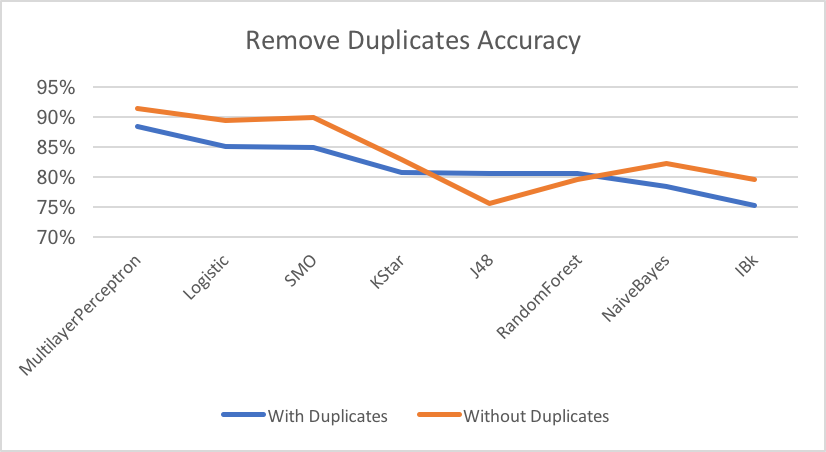
\includegraphics[width=150mm]{Figures/Duplicates.png}
\decoRule
\caption[Duplicates]{Landmark prediction accuracy with and without duplicate data points. Dataset Exeter Landmarks (see Section \ref{sec:ExeterDataset} and on \url{https://github.com/JoelNiklaus/IndoLoc/tree/master/app/src/main/assets/thesis/exeter/landmark})}
\label{fig:Duplicates}
\end{figure}

As we can clearly see in Table \ref{tab:Duplicates} and in a visualized way in Figure \ref{fig:Duplicates}, removing duplicate values increases the accuracy for most of the algorithms and especially for the ones that perform well. Of course, the computation time is decreased because the ML methods have less data points to consider. As a consequence, for all the following experiments duplicate values are removed.

We can see that after removing the duplicates the Multilayer Perceptron reaches a maximum landmark prediction accuracy of 91.41\%.

%----------------------------------------------------------------------------------------


%\section{Smaller Dataset}
%The \href{https://github.com/JoelNiklaus/IndoLoc/blob/master/app/src/test/java/ch/joelniklaus/indoloc/experiments/SmallerDataSetTest.java}{Smaller Dataset Test} checks if the accuracy is increased when only a randomly selected smaller part of the dataset is used. If this is the case, of course the performance is increased as well, because less data points have to be evaluated by the ML methods.
%
%
%
%% TABLE
%\begin{table}
%	\begin{threeparttable}
%		\caption{The accuracy change with randomly selected smaller datasets.}
%		\label{tab:SmallerDataset}
%		\centering
%		\begin{tabular}{l r r r r r r r}
%		\toprule
%		\tabhead{Classifier} & \tabhead{Full} & \tabhead{Half} & \tabhead{Third} & \tabhead{Fourth} & \tabhead{Fifth}  & \tabhead{Tenth} & \tabhead{Twentieth} \\
%		\midrule
%		MultilayerPerceptron		&	91.41\%	&	91.92\%	&	90.91\%	&	89.52\%	&	90.40\%	&	78.79\%	&	68.00\% \\%SMO	&	89.90\%	&	89.09\%	&	90.61\%	&	87.90\%	&	90.40\%	&	88.89\%	&	94.00\% \\%Logistic	&	89.29\%	&	88.89\%	&	90.61\%	&	88.71\%	&	88.89\%	&	80.81\%	&	90.00\% \\%NaiveBayes	&	82.12\%	&	80.61\%	&	83.03\%	&	82.26\%	&	85.35\%	&	90.91\%	&	92.00\% \\%IBk	&	79.49\%	&	77.78\%	&	80.61\%	&	78.23\%	&	79.80\%	&	77.78\%	&	88.00\% \\%RandomForest	&	79.49\%	&	79.80\%	&	83.03\%	&	82.66\%	&	83.33\%	&	81.82\%	&	90.00\% \\%J48	&	75.45\%	&	74.95\%	&	74.55\%	&	81.85\%	&	77.78\%	&	85.86\%	&	74.00\% \\
%		\bottomrule\\
%		\end{tabular}
%		\begin{tablenotes}
%      \small
%      \item Dataset: \href{https://github.com/JoelNiklaus/IndoLoc/tree/master/app/src/main/assets/thesis/exeter/landmark}{Exeter Landmarks}
%    \end{tablenotes}
%	\end{threeparttable}
%\end{table} \\
%
%% CHART
%\begin{figure}[th]
%\centering
%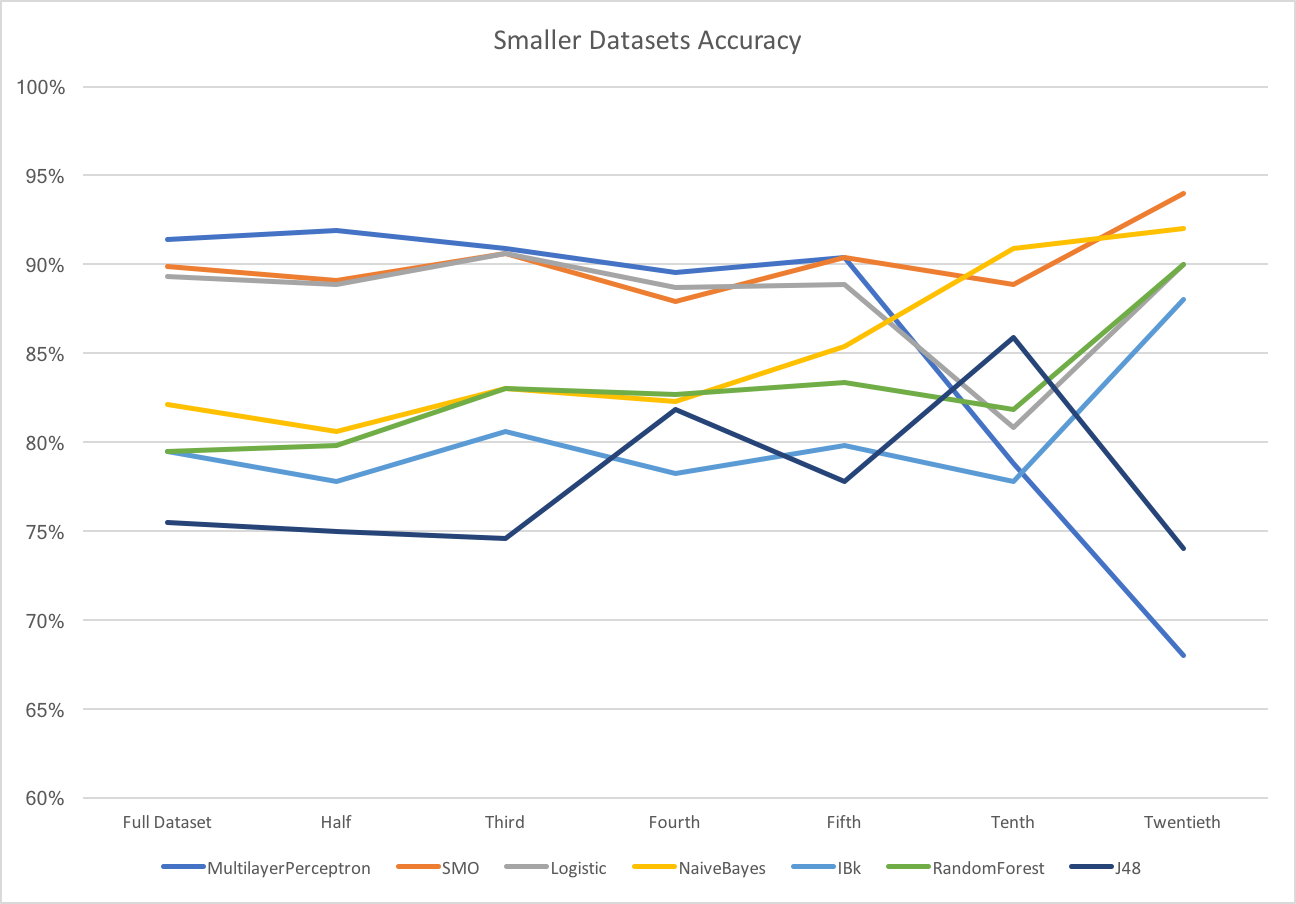
\includegraphics[width=150mm]{Figures/SmallerDataset.png}
%\decoRule
%\caption[SmallerDataset]{The accuracy change with randomly selected smaller datasets.}
%\label{fig:SmallerDataset}
%\end{figure}
%
%As we can see in Table \ref{tab:SmallerDataset} and Chart \ref{fig:SmallerDataset} the prediction accuracy is more or less stable until one third of the original size. In one fourth and one fifth of the size the accuracy decreases slightly. In one tenth and one twentieth of the size it starts to get erratic. So it probably depends on which data points are picked out of the original dataset. So for this dataset I would recommend to use one third of the data to slightly decrease the training and testing time. But the effect is minimal. 


%----------------------------------------------------------------------------------------

\section{Attribute Exclusion}
\label{sec:AttributeExclusion}

In Section \ref{sec:Features} we discussed which features seem reasonable to include into the dataset and which should be omitted because they do not seem helpful. In this section we test if the chosen features really all contribute to the prediction accuracy. To observe this, we selectively excluded certain features and studied the influences on the prediction accuracy.

This is done in the Attribute Exclusion Test (on  \url{https://github.com/JoelNiklaus/IndoLoc/blob/master/app/src/test/java/ch/joelniklaus/indoloc/experiments/AttributeExclusionTest.java}).

\subsection{Only RSS Values}

\subsubsection{Accuracy}


% TABLE
\begin{table}[H]
	\begin{threeparttable}
		\caption{The accuracy with a different number of RSS values.}
		\label{tab:RSSAccuracy}
		\centering
		\begin{tabular}{l r r r r r r}
		\toprule
		\tabhead{Classifier} & \tabhead{5 RSS} & \tabhead{6 RSS} & \tabhead{7 RSS} & \tabhead{8 RSS} & \tabhead{9 RSS}  & \tabhead{10 RSS} \\
		\midrule
		
		
		NaiveBayes &	82.05\%	&79.49\%	&	82.05\%	&	80.77\%	&	84.62\%	&	79.49\% \\IBk &	76.92\%	&	76.92\%	&	82.05\%	&	79.49\%	&	82.05\%	&	75.64\% \\KStar &	75.64\%	&	75.64\%	&	83.33\%	&	78.21\%	&	79.49\%	&	74.36\% \\SMO &	74.36\%	&	70.51\%	&	82.05\%	&	79.49\%	&	78.21\%	&	76.92\% \\Logistic &	73.08\%	&	66.67\%	&	73.08\%	&	66.67\%	&	71.79\%	&	69.23\% \\RandomForest &	71.79\%	&	71.79\%	&	79.49\%	&	75.64\%	&	73.08\%	&	75.64\% \\J48 &	64.10\%	&	57.69\%	&	64.10\%	&	64.10\%	&	64.10\%	&	64.10\% \\MultilayerPerceptron &	42.31\%	&	42.31\%	&	43.59\%	&	48.72\%	&	46.15\%	&	44.87\% \\
		\bottomrule\\
		\end{tabular}
		\begin{tablenotes}
      \small
      \item Dataset Bern Rooms (see Section \ref{sec:BernDataset} and on \url{https://github.com/JoelNiklaus/IndoLoc/tree/master/app/src/main/assets/thesis/bern/room}).
    \end{tablenotes}
	\end{threeparttable}
\end{table} 

% CHART
\begin{figure}[H]
\centering
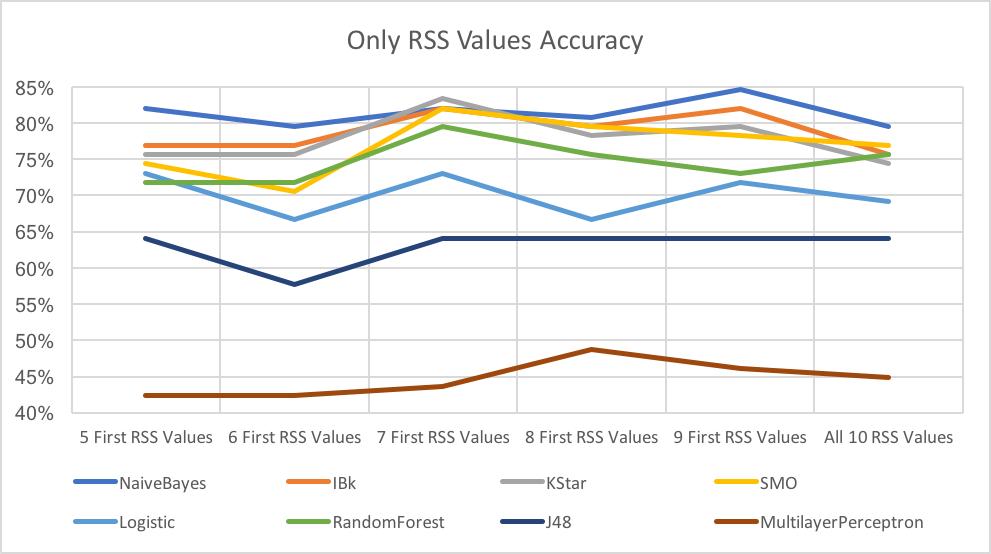
\includegraphics[width=150mm]{Figures/RssAccuracy.png}
\decoRule
\caption[RSSAccuracy]{The accuracy with a different number of RSS values. Dataset Bern Rooms (see Section \ref{sec:BernDataset} and on \url{https://github.com/JoelNiklaus/IndoLoc/tree/master/app/src/main/assets/thesis/bern/room})}
\label{fig:RSSAccuracy}
\end{figure}



Table \ref{tab:RSSAccuracy} and Figure \ref{fig:RSSAccuracy} show that there are two peaks, namely when 7 and 9 RSS values are used. The Naive Bayes classifier reaches a maximum prediction accuracy of 84.62\% with 9 RSS values. The other methods that perform well (KStar, SMO, Logistic and Randomforest) are considerably better with 7 RSS values. Table \ref{tab:RSSTestTime} depicts that there is not a great difference in testing time between 7 and 9 RSS values. Both would be viable options, but because more methods performed well with 7 RSS values and because Naive Bayes was never the best classifier on the final set in our tests, we are working with 7 RSS values in this dataset from now on.
We opine that signal interference may be the reason for worse performance when more than 7 RSS values are utilized.



\subsubsection{Testing Time}


% TABLE
\begin{table}[H]
	\begin{threeparttable}
		\caption{The testing time with a different number of RSS values measured in \textmu s per instance.}
		\label{tab:RSSTestTime}
		\centering
		\begin{tabular}{l r r r r r r}
		\toprule
		\tabhead{Classifier} & \tabhead{5 RSS} & \tabhead{6 RSS} & \tabhead{7 RSS} & \tabhead{8 RSS} & \tabhead{9 RSS}  & \tabhead{10 RSS} \\
		\midrule
		
		
		
NaiveBayes	&	108	&	201	&	150	&	106	&	83	&	173 \\IBk	&	283	&	231	&	262	&	230	&	294	&	297 \\KStar	&	863	&	1747	&	1095	&	1139	&	1285	&	1633 \\SMO	&	58	&	55	&	63	&	45	&	62	&	63 \\Logistic	&	20	&	24	&	21	&	22	&	23	&	28 \\RandomForest	&	31	&	39	&	46	&	20	&	38	&	34 \\J48	&	20	&	25	&	59	&	25	&	22	&	23 \\MultilayerPerceptron	&	9	&	10	&	11	&	10	&	7	&	12 \\
		
		\bottomrule\\
		\end{tabular}
		\begin{tablenotes}
      \small
      \item Dataset Bern Rooms (see Section \ref{sec:BernDataset} and on \url{https://github.com/JoelNiklaus/IndoLoc/tree/master/app/src/main/assets/thesis/bern/room}).
    \end{tablenotes}
	\end{threeparttable}
\end{table} 


% CHART
\begin{figure}[H]
\centering
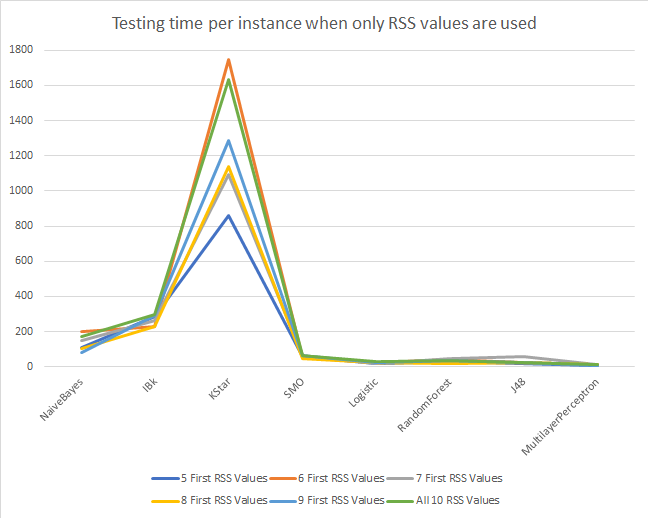
\includegraphics[width=150mm]{Figures/RssTestTime.png}
\decoRule
\caption[RSS Testing Time]{The testing time with a different number of RSS values measured in \textmu s per instance. Dataset Bern Rooms (see Section \ref{sec:BernDataset} and on \url{https://github.com/JoelNiklaus/IndoLoc/tree/master/app/src/main/assets/thesis/bern/room}).}
\label{fig:RSSTestTime}
\end{figure}

Testing time is defined as the time needed to classify an instance and is measured in \textmu s per instance. The tests have been conducted on a MacBook Pro, late 2013 edition with a 2.4 GHz Intel Core i5 CPU running macOS Sierra .

Table \ref{tab:RSSTestTime} and Figure \ref{fig:RSSTestTime} present that instance based methods like IBk (K-Nearest Neighbour) and especially KStar need so much more time than the other methods (IBk between 230 and 297 and KStar between 863 and 1747 microseconds per instance). This is because they have to look at the whole dataset each time an instance is classified, in contrast to other methods that use functions whose parameters are tweaked during the training phase. As a consequence, we excluded KStar from these big datasets (room recognition), because the experiment would take too long, which is not practical in a real scenario. However, for landmark recognition it makes sense to include it, because the datasets are normally much smaller.
The best testing time was achieved by the Multilayer Perceptron with predictions made in between 7 and 12 microseconds per instance.



%ANDERES PAPER ZITIEREN 





\subsection{RSS and Magnetic Field}

This section describes how the room prediction accuracy changes when we add the magnetic field (see Section \ref{sec:MagneticField}), stored in different ways, to the RSS values. 

% TABLE
\begin{table}[H]
	\begin{threeparttable}
		\caption{The accuracy with different ways of storing the magnetic field.}
		\label{tab:RSSAndMagnetic}
		\centering
		\begin{tabular}{l r r r r r}
		\toprule
		\tabhead{Classifier} & \tabhead{1} & \tabhead{2} & \tabhead{3} & \tabhead{4} & \tabhead{5} \\
		\midrule
		
SMO &	82.05\%	&	82.05\%	&	87.51\%	&	88.06\%	&	86.98\% \\IBk	& 82.05\%	&	82.05\%	&	85.57\%	&	85.21\%	&	83.71\% \\NaiveBayes	&	82.05\%	&	82.05\%	&	82.82\%	&	80.94\%	&	79.99\% \\RandomForest	&	79.49\%	&	78.21\%	&	78.22\%	&	80.89\%	&	72.25\% \\Logistic	&	73.08\%	&	73.08\%	&	78.64\%	&	68.62\%	&	73.21\% \\J48	&	64.1\%	&	64.10\%	&	71.27\%	&	71.27\%	&	71.27\% \\MultilayerPerceptron	&	43.59\%	&	39.74\%	&	68.30\%	&	68.40\%	&	79.81\% \\
		
		\bottomrule\\
		\end{tabular}
	\begin{tablenotes}
      \small
      \item Dataset Bern Rooms (see Section \ref{sec:BernDataset} and on \url{https://github.com/JoelNiklaus/IndoLoc/tree/master/app/src/main/assets/thesis/bern/room}).
        \item Legend:
\item[1] 7 first RSS values
\item[2] RSS and gravityRaw and magneticRaw
\item[3] RSS and magneticProcessed
\item[4] RSS and gravityMagnitude and geomagneticMagnitude
\item[5] RSS and magneticProcessed and gravityMagnitude and geomagneticMagnitude
      
    \end{tablenotes}
	\end{threeparttable}
\end{table} 

% CHART
\begin{figure}[H]
\centering
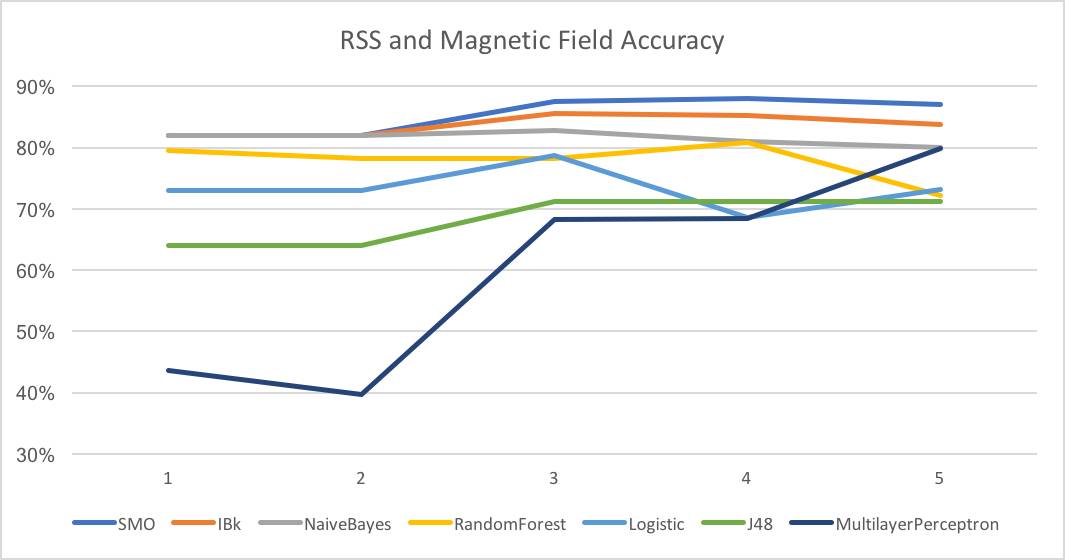
\includegraphics[width=150mm]{Figures/RSSAndMagnetic.png}
\decoRule
\caption[RSSAndMagnetic]{The accuracy with different ways of storing the magnetic field. Dataset Bern Rooms (see Section \ref{sec:BernDataset} and on \url{https://github.com/JoelNiklaus/IndoLoc/tree/master/app/src/main/assets/thesis/bern/room}).}
\label{fig:RSSAndMagnetic}
	
	\begin{threeparttable}
    \begin{tablenotes}
  \item Legend:
\item[1] 7 RSS values
\item[2] RSS and gravityRaw and magneticRaw
\item[3] RSS and magneticProcessed
\item[4] RSS and gravityMagnitude and geomagneticMagnitude
\item[5] RSS and magneticProcessed and gravityMagnitude and geomagneticMagnitude
    \end{tablenotes}
	\end{threeparttable}

\end{figure}


%TABLES AND CHARTS SHOULD APPEAR AT THE RIGHT PLACE

%EXPLAIN HOW EXACTLY VALUES ARE COMPUTED VERWEIS AUF THEORIE

Table \ref{tab:RSSAndMagnetic} and Figure \ref{fig:RSSAndMagnetic} indicate that adding the raw values of the gravity and magnetic field (2) does not improve the accuracy . Adding the magneticProcessed values (3) improves prediction accuracy for most of the algorithms and by 5\% for the best performing method SMO (Sequential Minimal Optimization), for example. Adding the gravity magnitude and the geomagnetic magnitude instead of magneticProcessed (4), some methods perform better and some worse. SMO for instance still improves, but Logistic Regression gets worse. Adding both of the last two at the same time, (5) we could expect that the effect is combined. But interestingly, the accuracy of the top performing methods decreases again. On the other hand, the MultilayerPerceptron performs much better. 
The best room prediction accuracy is reached by the SMO classifier with 88.06\% using RSS values, gravityMagnitude and geomagneticMagnitude




\subsection{Additional Features}
\label{AdditionalFeatures}

This section describes how the room prediction accuracy changes, when we add additional features, namely light and GPS data, to the dataset.

% TABLE
\begin{table}[H]
	\begin{threeparttable}
		\caption{The accuracy with additional features added.}
		\label{tab:AdditionalFeatures}
		\centering
		\begin{tabular}{l r r r}
		\toprule
		\tabhead{Classifier} & \tabhead{1} & \tabhead{2} & \tabhead{3} \\
		\midrule
		
SMO &	86.98\%	&	88.02\%	&	84.16\% \\IBk	& 83.71\%	&	84.74\%	&	81.1\% \\NaiveBayes &	79.99\%	&	90.13\%	&	44.12\% \\MultilayerPerceptron &	79.81\%	&	73.16\%	&	44.93\% \\Logistic &	73.21\%	&	71.81\%	&	55.77\% \\RandomForest &	72.25\%	&	82.33\%	&	41.55\% \\J48 &	71.27\%	&	76.57\%	&	35.65\% \\
				
		\bottomrule\\
		\end{tabular}
		\begin{tablenotes}
      \small
      \item Dataset Bern Rooms (see Section \ref{sec:BernDataset} and on \url{https://github.com/JoelNiklaus/IndoLoc/tree/master/app/src/main/assets/thesis/bern/room}).
      \item Legend:
      \item[1] RSS and magneticProcessed and gravityMagnitude and geomagneticMagnitude
\item[2] RSS and magneticProcessed and gravityMagnitude and geomagneticMagnitude and Light
\item[3] RSS and magneticProcessed and gravityMagnitude and geomagneticMagnitude and Latitude and Longitude
    \end{tablenotes}
	\end{threeparttable}
\end{table} 

% CHART
\begin{figure}[H]
\centering
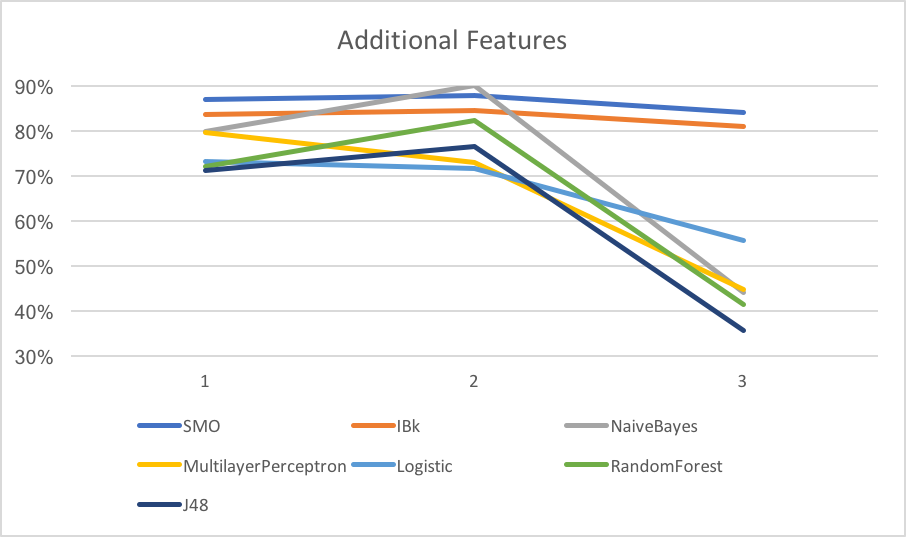
\includegraphics[width=150mm]{Figures/AdditionalFeatures.png}
\decoRule
\caption[AdditionalFeatures]{The accuracy with additional features added. Dataset Bern Rooms (see Section \ref{sec:BernDataset} and on \url{https://github.com/JoelNiklaus/IndoLoc/tree/master/app/src/main/assets/thesis/bern/room}).}
\label{fig:AdditionalFeatures}

\begin{threeparttable}
\begin{tablenotes}
      \item Legend:
      \item[1] RSS and magneticProcessed and gravityMagnitude and geomagneticMagnitude
\item[2] RSS and magneticProcessed and gravityMagnitude and geomagneticMagnitude and Light
\item[3] RSS and magneticProcessed and gravityMagnitude and geomagneticMagnitude and Latitude and Longitude
    \end{tablenotes}
	\end{threeparttable}

\end{figure}



% CONFUSION MATRIX
\begin{table}[H]
\caption{The confusion matrix for the Naive Bayes classifier using the dataset number 2 (with light). Dataset Bern Rooms (see Section \ref{sec:BernDataset} and on \url{https://github.com/JoelNiklaus/IndoLoc/tree/master/app/src/main/assets/thesis/bern/room}).}
\label{ver:ConfusionMatrix}

\begin{verbatim}
    1    2    3    4    5    6    7    8    9   <-- classified as
----------------------------------------------+
 2145    0    0    0   19    0    0    0    0 |    1
    0  640    0    0    0    0    0   25    0 |    2
    0  104  786    0    0    0    0    0    0 |    3
    0  112    0  137    0    0    0   42    0 |    4
   77    0   45    0  507    0    0   56    0 |    5
    0    0  101    0    0 1217    0    0    0 |    6
    0   73    3    0    0    0  984    0   11 |    7
    0    3    0  116    0    0    0  528    0 |    8
    0    0    0    0    0    0    0   64  829 |    9
\end{verbatim}
\end{table}


Table \ref{tab:AdditionalFeatures} and Figure \ref{fig:AdditionalFeatures} depict that adding Light comes with an improvement for most tested methods. The Naive Bayes classifier even reaches an accuracy of 90.13\% using RSS values, magneticProcessed, gravitiyMagnitude, geomagneticMagnitude and Light (for more information concerning data collection see Section  \ref{sec:DataCollection}).
%But here we should additionally test if this improvement still holds for a testing set collected in the night for instance (see in conclusion \ref{light}). 
%But adding the latitude and longitude values obtained from the GPS seems to only confuse the algorithms apparently. This is probably because the values are just so inaccurate and no more than noise. But the goal of this project is to be independent from GPS indoors.

A confusion matrix is a table with the classification of the ML algorithm in the column and the actual class in the row. So if an instance gets classified as class 2 but actually belongs to class 4, the value at the respective coordinates in the table is incremented by one. This is done for all of the instances in the test set. So on the main diagonal from the top left corner to the bottom right corner there are all the correctly classified instances. On all the other places in the table we can see the incorrectly classified instances. 
The confusion matrix gives very interesting insights into the problems of the classifiers. It tells us which classes the classifier mixes up. We can see how many instances have been assigned a certain class (column head) by the ML method and what their actual class (row head (to the right)) is. An example for a confusion matrix is shown in Table \ref{ver:ConfusionMatrix}.

In the confusion matrix, shown in Table \ref{ver:ConfusionMatrix}, it is clearly visible that the classifier has problems with class 2 (the corridor), because many values are not situated on the main diagonal but instead in column and row 2. The classifier often confuses class 2 with the classes 3, 4 and 7. These are some of the smaller rooms, as can be seen in Figure \ref{fig:Bern}. It also struggles with predicting class 3 and 8 correctly. 
Room 6, 7 and to some extent 5 and 9 seem to be 'weak' classes as it (almost) never happens that the classifier selects one of these classes, when it actually was another class. The opposite, namely that the classifier selects another class when it actually was one of these classes, happens sometimes.
For the rooms 1 and 2 the opposite applies. A data point which is in one of these rooms very seldom gets classified as another class. So these two seem to be 'strong' classes. The classifier seems to like these classes.




%----------------------------------------------------------------------------------------

\section{Rounding}
\label{sec:Rounding}
Some sensors return values with more than 5 decimal places although they are less accurate than 0.1. Because of this, we considered rounding these values to the respective measuring accuracy of the sensor in order to reduce the size of the dataset.

The Rounding Test (on \url{https://github.com/JoelNiklaus/IndoLoc/blob/master/app/src/test/java/ch/joelniklaus/indoloc/experiments/RoundingTest.java}) checks if the accuracy is increased, when some features containing decimal places are rounded. We performed tests on the dataset reduced to 7 RSS values, magneticProcessed, gravityMagnitude and geomagneticMagnitude. We performed tests where we rounded with accuracy integer, 0.2 and 0.1. However, prediction accuracy did not increase for any of the tests.


%----------------------------------------------------------------------------------------


\section{Hyper-Parameter Search}
\label{sec:HyperParameterSearch}
The Hyperparameter Search Test (on \url{https://github.com/JoelNiklaus/IndoLoc/blob/master/app/src/test/java/ch/joelniklaus/indoloc/experiments/HyperParameterSearchTest.java} checks if the accuracy is increased when certain parameters from the ML methods are changed. Hyper-Parameter search can be done with algorithms like grid search, multisearch and auto-weka for instance. It can also be done by trial and error. Using these methods we evaluated several classifiers on the train\_optimal and test\_optimal datasets (on  \url{https://github.com/JoelNiklaus/IndoLoc/tree/master/app/src/main/assets/thesis/bern/room/}). Here we used the first 9 RSS values, the magneticProcessed, geomagneticMagnitude, gravityMagnitude and light features. The three best performing algorithms are the Multilayer Perceptron with an accuracy of 92.08 \%, shown in Table \ref{ver:ConfusionMatrixMultilayerPerceptron}, the Sequential Minimal Optimization with an accuracy of 89.24 \%, presented in Table \ref{ver:ConfusionMatrixSMO} and the Naive Bayes classifier with an accuracy of 89.61 \%, depicted in Table \ref{ver:ConfusionMatrixNaiveBayes}.

% CONFUSION MATRIX
\begin{table}[H]
\caption{The confusion matrix for the MultilayerPerceptron classifier. Dataset Bern Rooms (see Section \ref{sec:BernDataset} and on \url{https://github.com/JoelNiklaus/IndoLoc/tree/master/app/src/main/assets/thesis/bern/room}).}
\label{ver:ConfusionMatrixMultilayerPerceptron}
\begin{threeparttable}
\begin{verbatim}
    a    b    c    d    e    f    g    h    i   <-- classified as
 2164    0    0    0    0    0    0    0    0 |    a = 1
    0  527    0    0    0    0    0    0  138 |    b = 2
    0   25  865    0    0    0    0    0    0 |    c = 3
    0    9    0  154    0    0    0  128    0 |    d = 4
    0   43    0    0  642    0    0    0    0 |    e = 5
    0   25    0    0   44 1249    0    0    0 |    f = 6
    0    6    0    0    0    0 1064    0    1 |    g = 7
    0    0    0  149    0    0    0  498    0 |    h = 8
    0    0    0   51    0    0    0   64  778 |    i = 9
\end{verbatim}
\begin{tablenotes}
\item Accuracy: 92.0802 \% 
\item Parameters:
\tiny{
\begin{verbatim}
weka.classifiers.functions.MultilayerPerceptron -L 0.2 -M 0.1 -N 40 -V 0 -S 0 -E 20 -H a -batch-size 100
\end{verbatim}
}
\end{tablenotes}
\end{threeparttable}
\end{table}



% CONFUSION MATRIX
\begin{table}[H]
\caption{The confusion matrix for the SMO classifier. Dataset Bern Rooms (see Section \ref{sec:BernDataset} and on \url{https://github.com/JoelNiklaus/IndoLoc/tree/master/app/src/main/assets/thesis/bern/room}).}
\label{ver:ConfusionMatrixSMO}
\begin{threeparttable}
\begin{verbatim}
    a    b    c    d    e    f    g    h    i   <-- classified as
 2164    0    0    0    0    0    0    0    0 |    a = 1
   10  632    0    0    0    0    0    0   23 |    b = 2
    0   55  799    0    0   36    0    0    0 |    c = 3
    0  147    0  144    0    0    0    0    0 |    d = 4
    0   43    0    0  642    0    0    0    0 |    e = 5
  204   69   32    0    0 1013    0    0    0 |    f = 6
    0  126    0    0    0    0  945    0    0 |    g = 7
    0    0    0  119    0    0    0  528    0 |    h = 8
    0    0    0   57    0    0    0    7  829 |    i = 9
\end{verbatim}
\begin{tablenotes}
\item Accuracy: 89.2393 \%
\item Parameters:
\tiny{
\begin{verbatim}
weka.classifiers.functions.SMO -C 1.0 -L 0.001 -P 1.0E-12 -N 0 -V -1 -W 1 -K
    "weka.classifiers.functions.supportVector.PolyKernel -E 1.0 -C 250007" -calibrator
    "weka.classifiers.functions.Logistic -R 1.0E-8 -M -1 -num-decimal-places 4"
\end{verbatim}
}
\end{tablenotes}
\end{threeparttable}
\end{table}


% CONFUSION MATRIX
\begin{table}[H]
\caption{The confusion matrix for the Naive Bayes classifier. Dataset Bern Rooms (see Section \ref{sec:BernDataset} and on \url{https://github.com/JoelNiklaus/IndoLoc/tree/master/app/src/main/assets/thesis/bern/room}).}
\label{ver:ConfusionMatrixNaiveBayes}
\begin{threeparttable}
\begin{verbatim}
    a    b    c    d    e    f    g    h    i   <-- classified as
 2149    0    0    0   15    0    0    0    0 |    a = 1
    0  393    9  153    0    0    0  110    0 |    b = 2
    0    0  876    0    0   14    0    0    0 |    c = 3
    0  130    0  135    0    0    0   26    0 |    d = 4
    1    0   44    0  628    0    0   12    0 |    e = 5
    0    0  101    0    0 1217    0    0    0 |    f = 6
    0   59   12    0    0    0  973    0   27 |    g = 7
    0    0    0  119    0    0    0  528    0 |    h = 8
    0    0    0    0    0    0    0   64  829 |    i = 9
\end{verbatim}
\begin{tablenotes}
\item Accuracy: 89.6104 \%
\item Parameters:
\tiny{
\begin{verbatim}
weka.classifiers.bayes.NaiveBayes
\end{verbatim}
}
\end{tablenotes}
\end{threeparttable}
\end{table}

When we analyze the confusion matrices of these three classifers we derive the following observations: the Multilayer Perceptron is very good in column b as compared to the other two; SMO is very good in the triangle above the diagonal; and Naive Bayes has its own problems specially distributed but performs well at other places where the other two are bad (i2 or b5 for instance). This diversity can be used by meta classifiers (ensemble learning methods) which is described in Section \ref{sec:Ensemble}.

%----------------------------------------------------------------------------------------


\section{Optimal Prediction With Ensemble Methods}
\label{sec:Ensemble}
Ensemble methods combine several base classifiers into one in order to improve the prediction accuracy.

The Optimal Prediction Test (on  \url{https://github.com/JoelNiklaus/IndoLoc/blob/master/app/src/test/java/ch/joelniklaus/indoloc/experiments/OptimalPredictionTets.java}) edits the dataset in a certain way and configures the ML algorithm with parameters in such a way that the accuracy is optimized. This is based on the knowledge out of the previous tests or previous experiences.

We tried the following different ensemble methods: Grading, Stacking, Decorate, Boosting, Bagging, Dagging and RandomSubSpace, all using SMO as the base classifier. However, none of the ensemble learning methods significantly improved the prediction accuracy. In addition, by combining several different classifiers using voting we achieved a better prediction accuracy, as shown in Table \ref{ver:ConfusionMatrixMajorityVote}. Voting is an ensemble method which evaluates several different base ML algorithms and then usually combines the results using majority vote.

% CONFUSION MATRIX
\begin{table}[H]
\caption{The confusion matrix for the Majority Vote classifier with three MultilayerPerceptrons, a ClasssificationViaRegression, a RandomSubspace, a LogitBoost, a RandomForest,  a Logistic Regression,  a SMO and a Naive Bayes classifier. Dataset Bern Rooms (see Section \ref{sec:BernDataset} and on \url{https://github.com/JoelNiklaus/IndoLoc/tree/master/app/src/main/assets/thesis/bern/room}).}
\label{ver:ConfusionMatrixMajorityVote}
\begin{threeparttable}
\begin{verbatim}
    a    b    c    d    e    f    g    h    i   <-- classified as
 2164    0    0    0    0    0    0    0    0 |    a = 1
    0  663    0    0    0    0    0    0    2 |    b = 2
    0   25  865    0    0    0    0    0    0 |    c = 3
    0   32    0  143    0    0    0  116    0 |    d = 4
    0   43    0    0  642    0    0    0    0 |    e = 5
    0   69    0    0    0 1249    0    0    0 |    f = 6
    0   43    0    0    0    0 1027    0    1 |    g = 7
    0    0    0  119    0    0    0  528    0 |    h = 8
    0    0    0    0    0    0    0   64  829 |    i = 9
\end{verbatim}
\begin{tablenotes}
\item Accuracy: 94.0399 \%
\item Parameters:
\tiny{
\begin{verbatim}
weka.classifiers.meta.Vote -S 1 -B
    "weka.classifiers.functions.MultilayerPerceptron -L 0.4 -M 0.3 -N 100 -V 0 -S 0 -E 20 -H a" -B
    "weka.classifiers.functions.MultilayerPerceptron -L 0.3 -M 0.2 -N 100 -V 0 -S 0 -E 20 -H a" -B
    "weka.classifiers.functions.MultilayerPerceptron -L 0.2 -M 0.1 -N 40 -V 0 -S 0 -E 20 -H a" -B
    "weka.classifiers.functions.MultilayerPerceptron -L 0.2 -M 0.1 -N 40 -V 0 -S 0 -E 20 -H a" -B
    "weka.classifiers.meta.RandomSubSpace -P 0.5 -S 1 -num-slots 1 -I 10 -W
        weka.classifiers.trees.REPTree -- -M 2 -V 0.001 -N 3 -S 1 -L -1 -I 0.0" -B
    "weka.classifiers.meta.LogitBoost -P 100 -L -1.8E308 -H 1.0 -Z 3.0 -O 1 -E 1 -S 1 -I 10 -W
        weka.classifiers.trees.DecisionStump" -B
    "weka.classifiers.trees.RandomForest -P 100 -I 100 -num-slots 1 -K 0 -M 1.0 -V 0.001 -S 1" -B
    "weka.classifiers.functions.Logistic -R 1.0E-8 -M -1 -num-decimal-places 4" -B
    "weka.classifiers.functions.SMO -C 1.0 -L 0.001 -P 1.0E-12 -N 0 -V -1 -W 1 -K
    "weka.classifiers.functions.supportVector.PolyKernel -E 1.0 -C 250007" -calibrator
    "weka.classifiers.functions.Logistic -R 1.0E-8 -M -1 -num-decimal-places 4" -B
    "weka.classifiers.bayes.NaiveBayes"
    -R MAJ
\end{verbatim}
}
\end{tablenotes}
\end{threeparttable}
\end{table}

We can see that the room prediction accuracy could be improved by almost 2\% to 94.0399\% over the the best base classifier (the Multilayer Perceptron) with 92.0802\%. This is a large improvement on this level.

Looking at the confusion matrices, shown in Tables \ref{ver:ConfusionMatrixMultilayerPerceptron}, \ref{ver:ConfusionMatrixSMO}, \ref{ver:ConfusionMatrixNaiveBayes} and \ref{ver:ConfusionMatrixMajorityVote} we can also see that the voting classifier, depicted in Table \ref{ver:ConfusionMatrixMajorityVote}, adopted some behaviour of some classifiers and other behaviour of others. In general, for instance, it adopted the good behaviour of the Multilayer Perceptron, depicted in Table \ref{ver:ConfusionMatrixMultilayerPerceptron}, in column b. However, it does not make the mistake in i2 (column i, row 2) anymore but it adopted the good behaviour of the Naive Bayes classifier, shown in Table \ref{ver:ConfusionMatrixNaiveBayes}. Unfortunately, it still has the problems at h4 probably originating from the Multilayer Perceptron, shown in Table \ref{ver:ConfusionMatrixMultilayerPerceptron}. If we gave more weight to the SMOs prediction, shown in Table \ref{ver:ConfusionMatrixSMO}, for instance (not having this problem at h4) it would probably resolve this issue but the prediction accuracy in column b would deteriorate again. In general, it can be seen that it seems difficult to distinguish the rooms 4 and 8, which are two small rooms next to each other, as depicted in Figure \ref{fig:Bern}.

%This is a never ending process though, but given more time it is probably possible to achieve even higher accuracy by tweaking the parameters.

%----------------------------------------------------------------------------------------


 
% Chapter 5

\chapter{Conclusions and Future Directions} % Main chapter title
\label{Chapter5} % For referencing the chapter elsewhere, use \ref{Chapter5} 


%----------------------------------------------------------------------------------------

In this chapter we conclude the main contributions and findings of this thesis and over the entire project and give ideas for future work in this area. 


\section{Conclusion}
In this thesis we first developed an Android app, which is able to collect data of the phone's surroundings. This data comprises of the RSS values of the nearby WiFi access points, of information about the earth's magnetic and gravity field and of sensor information, namely pressure, ambient temperature, relative humidity and light. The application is further able to train several ML methods to distinguish between different rooms and landmarks (specified areas within rooms).
Second, we collected data in order to analyze and then optimize the performance of the chosen ML algorithms.

For room recognition in the dataset taken in the INF building in Bern (see Section \ref{sec:BernDataset}), distinguishing between 9 different rooms we achieved the following results:
A Multilayer Perceptron, the best base classifier, reached an accuracy of 92.08\% (see evaluation \ref{ver:ConfusionMatrixMultilayerPerceptron}). Combining several base learners using Majority Vote (namely three MultilayerPerceptrons, a ClasssificationViaRegression, a RandomSubspace, a LogitBoost, a RandomForest,  a Logistic Regression,  a SMO and a Naive Bayes classifier) we could reach a maximal accuracy of even 94.0399 \% (see evaluation \ref{ver:ConfusionMatrixMajorityVote}). For landmark recognition in the dataset taken in student accommodation in Exeter (see Section \ref{sec:ExeterDataset}) distinguishing between 5 different landmarks we achieved 91.41\% accuracy using a Multilayer Perceptron. 

Because of these very high accuracies in both room and landmark recognition we are confident that this approach using machine learning can improve the ITS. 

%----------------------------------------------------------------------------------------

\section{Future Directions}

\subsection{Device Independence}
In the experiments done in the scope of this project, we collected the training and the testing data sets on the same phone. Different hardware measuring the environment differently could make the accuracy deteriorate vastly. This could be tested with various current smart phones.

One solution for this problem could be data normalization. For instance, we would not store the RSS values directly, but compute the difference to a representative starting point and normalize the result to a value between 0 and 1. 

\subsection{Only Predict if Sure}
An idea to improve the security of a prediction would be to only forward a prediction from Indoloc to the ITS if the Indoloc system is sure (probability greater than some defined threshold). In this way we could ensure that almost no wrong predictions are made which could confuse the ITS. But of course, it would also come with less predictions over all. And it still has to be tested if false predictions are (almost) only made when the Indoloc system is not sure.


\subsection{Further Optimization of HyperParameters}
As already discussed, it is very difficult to find optimal hyperparameters for the ML methods. Further testing could be done to optimize these.


\subsection{Longterm Stability}
As described in Section \ref{WiFiAndSensorData}, no test about longterm stability has been done yet. So it has to be tested if a model trained with data collected at point A is still performing well enough a month, a year or even more later. 

\subsection{Light}
\label{light}
As described in the results of Section \ref{AdditionalFeatures}, the light feature improves the accuracy for most algorithms. But in the night, or if it is a cloudy day, or in a different season or under some other different condition, it probably decreases the accuracy. 

A possible solution for this would be the following: we only consider the relative light difference between the different rooms or landmarks respectively. \\
But of course if we detect that the proportionalities of the light strengths in the rooms or landmarks respectively are not similar under some circumstances it does not make sense to include the light feature at all!


\subsection{Bluetooth}
By using specially installed Bluetooth beacons at the borders of the room (predominantly doors) we hope to further improve the accuracy of the ITS because that is where Indoloc has the greatest problems identifying the correct room. 

\subsection{RSS Values}
As described in Section \ref{sec:RSS} we collected the RSS values of all the nearby access points. A value lower than -80 is very weak and may suggest that the access point is very far away or there are many or big obstacles between the access point and the collecting device. This means that the access point is of little or no use to the system. Therefore, we could remove access points with values smaller than -80 from the list in a future version.



%---------------------------------------------------------------------------------------- 

%----------------------------------------------------------------------------------------
%	THESIS CONTENT - APPENDICES
%----------------------------------------------------------------------------------------

\appendix % Cue to tell LaTeX that the following "chapters" are Appendices

% Include the appendices of the thesis as separate files from the Appendices folder
% Uncomment the lines as you write the Appendices

%% Appendix A

\chapter{Results} % Main appendix title

\label{AppendixA} % For referencing this appendix elsewhere, use \ref{AppendixA}

\section{Tables}
%% Appendix B

\chapter{asdf} % Main appendix title

\label{AppendixB} % For referencing this appendix elsewhere, use \ref{AppendixB}

\section{ads}
%% Appendix C

\chapter{asdf} % Main appendix title

\label{AppendixC} % For referencing this appendix elsewhere, use \ref{AppendixC}

\section{ads}
%% Appendix X

\chapter{Frequently Asked Questions} % Main appendix title

\label{AppendixX} % For referencing this appendix elsewhere, use \ref{AppendixX}

\section{How do I change the colors of links?}

The color of links can be changed to your liking using:

{\small\verb!\hypersetup{urlcolor=red}!}, or

{\small\verb!\hypersetup{citecolor=green}!}, or

{\small\verb!\hypersetup{allcolor=blue}!}.

\noindent If you want to completely hide the links, you can use:

{\small\verb!\hypersetup{allcolors=.}!}, or even better: 

{\small\verb!\hypersetup{hidelinks}!}.

\noindent If you want to have obvious links in the PDF but not the printed text, use:

{\small\verb!\hypersetup{colorlinks=false}!}.
 % template

%----------------------------------------------------------------------------------------
%	BIBLIOGRAPHY
%----------------------------------------------------------------------------------------

\printbibliography[heading=bibintoc]


%----------------------------------------------------------------------------------------
%	ERKLAERUNG
%----------------------------------------------------------------------------------------

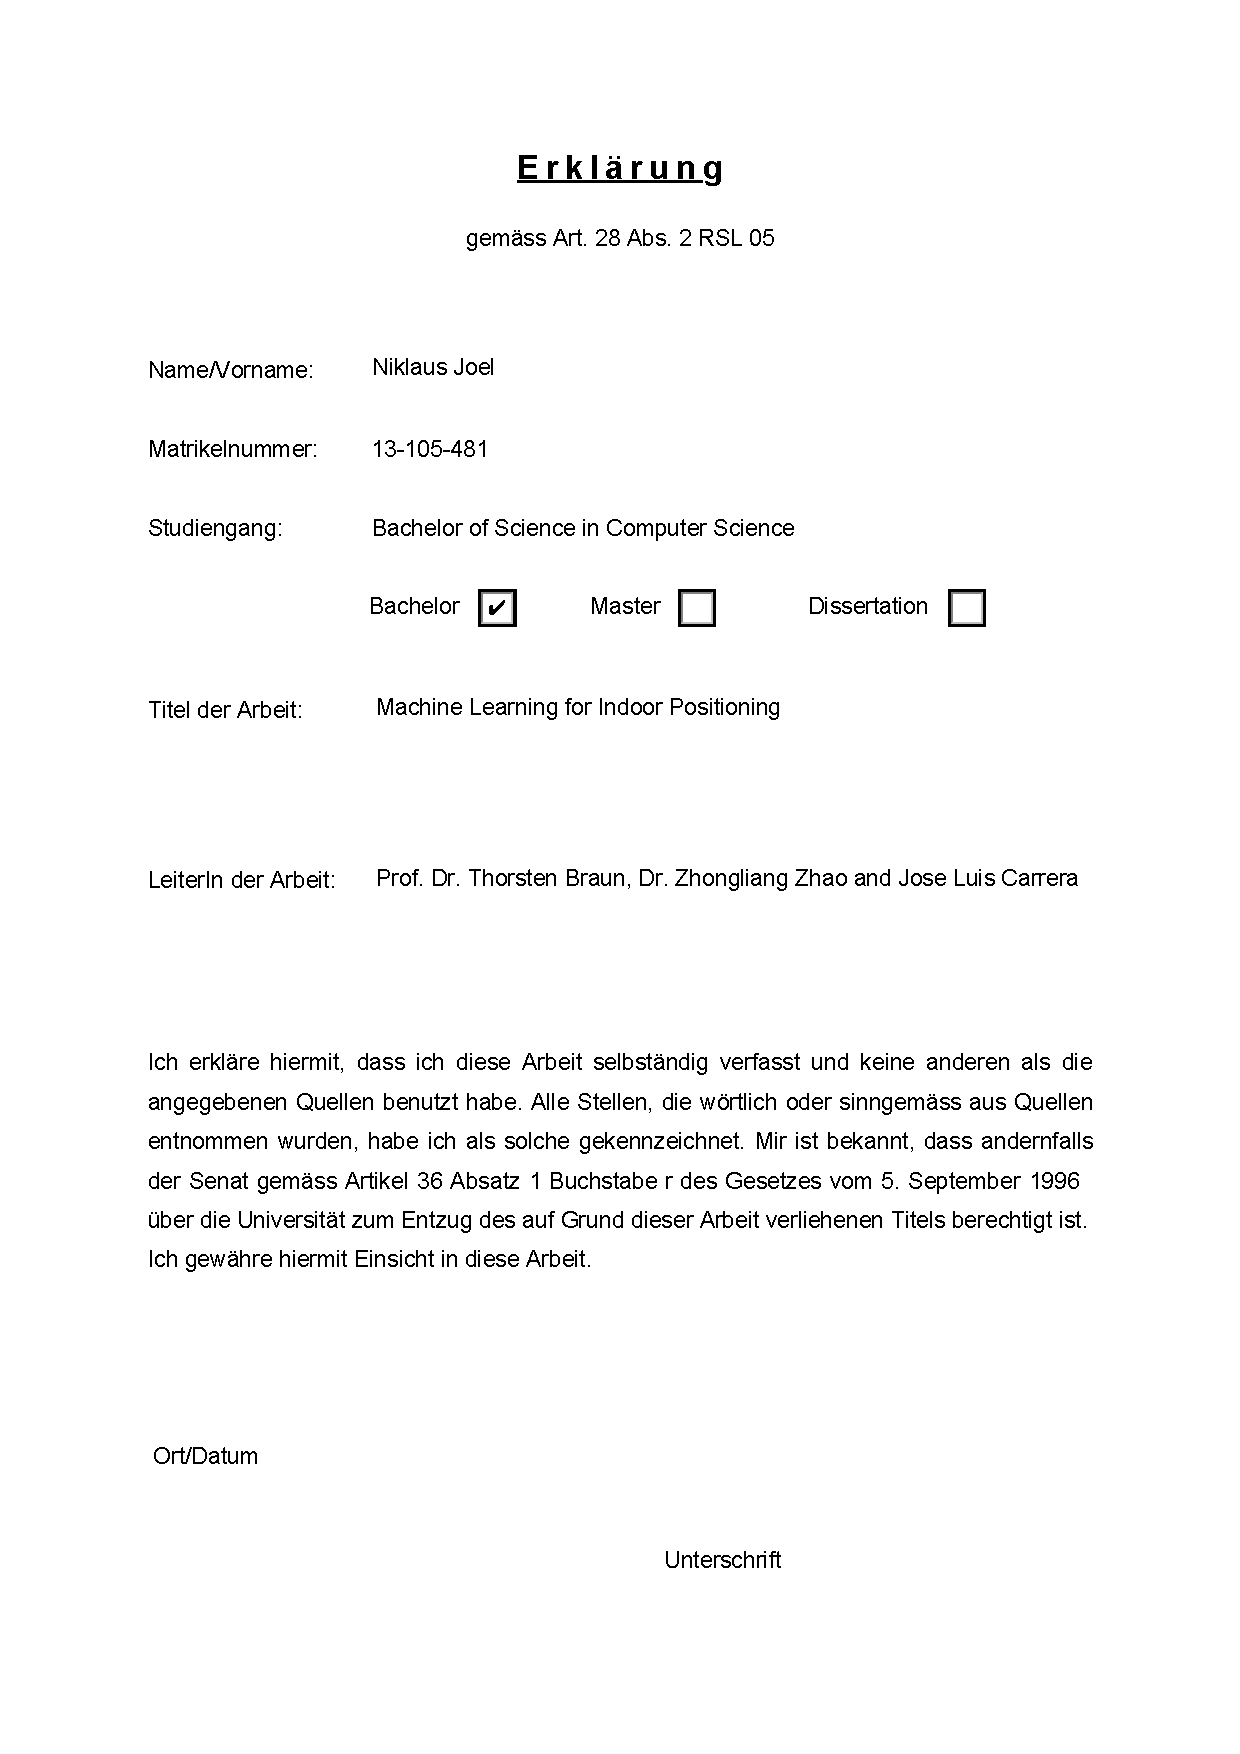
\includepdf{BSc_bachelorarbeit_erklaerung.pdf}

%----------------------------------------------------------------------------------------


\end{document}  
